% !TeX encoding = UTF-8
% !TeX program = xelatex
% !TeX spellcheck = en_US

\documentclass[doctor,english,pdf]{ustcthesis}
% doctor|master|bachelor [academic|professional] [chinese|english] [print|pdf]
% [super|numebers|authoryear]

\title{利用ATLAS探测器上ZZ 玻色子到全轻子通道的衰变事例进行电弱对称性破缺的研究}
\author{祝鹤龄}
%\major{粒子与原子核物理}
\supervisor{赵政国}
\cosupervisor{马宏}
% \date{二〇一七年五月一日} % 注释掉则为今日
% \professionaltype{专业学位类型}
% \secretlevel{秘密}        % 绝密|机密|秘密,注释本行则不保密
% \secretyear{20}           % 保密年限

\entitle{Study of Electroweak Symmetry Breaking in ZZ Production in Purely Leptonic Decay with ATLAS Detector}
\enauthor{Heling Zhu}
%\enmajor{Particle and Nuclear Physics}
\ensupervisor{Zhengguo Zhao}
\encosupervisor{Hong Ma}
% \endate{May 1, 2017}      % Today if commented
% \enprofessionaltype{Professional degree type}
% \ensecretlevel{Secret}    % Top secret|Highly secret|Secret


% 加载宏包和配置
\usepackage{graphicx}
\graphicspath{{figures/}}
\usepackage{booktabs}
\usepackage{longtable}
\usepackage[ruled,linesnumbered]{algorithm2e}
\usepackage{siunitx}
\usepackage{amsthm}
\usepackage{hyperref}

\DeclareRobustCommand\cs[1]{\texttt{\char`\\#1}}
\newcommand\pkg{\textsf}

\renewcommand\vec{\symbf}
\newcommand\mat{\symbf}
\newcommand\ts{\symbfsf}
\newcommand\real{\mathbf{R}}
%\newcommand{\doi}[1]{\textsc{doi}: \href{http://dx.doi.org/#1}{\nolinkurl{#1}}}
\newcommand{\doi}[1]{\href{http://dx.doi.org/#1}{\nolinkurl{#1}}}


\begin{document}

% 研究生论文:
%   封面,原创性声明和授权使用声明
%   frontmatter: 摘要,目录,[图、表清单],[符号说明]
%   mainmatter: 正文章节,参考文献
%   appendix: 附录
%   backmatter: 致谢,已发表论文列表

\maketitle
\makestatement

\frontmatter
% !TeX root = ../main.tex

\begin{abstract}
  中文摘要
\end{abstract}

\begin{enabstract}
  English abstract.

\end{enabstract}

% !TeX root = ../main.tex

\begin{acknowledgments}

First of all, I would like to express my great gratitude to my supervisors Prof. Zhao Zhengguo and Dr. Ma Hong, for their guidance and patience during my Ph.D years.
It's Zhengguo, who inspire me with his deep physics insight when I was an undergraduate student and led me enter the field of Particle Physics.
I will never forget how I was attracted by his broad knowledge and the amazing picture of particles he showed me, which became the reason I choose the Particle Physics as my major.
It's always relaxed and benificial greatly when chating with him, which broads my version, makes me to be more confident and helps me step out of so many difficulties.

Thanks to Hong, for giving me the oppotunity to study in Brookhaven National Lab (BNL) that I can work with so many senior and brilliant physicists, and teaching me a lot in the details of physics.
As the chair of physics department at BNL, can you imagine that he managed to take time sitting with me every week, teaching me the details and techniques of my analysis
as well as helping me to parepre my talks at conference.

Thank you both for leading me to the field of physics, showing me how beautiful the science and the world are. 
And thank you for providing me so many oppotunities and tremendous supports to work at physics frontier and work with people all over the world.
It's my greatest honor to be your student.
Your strong personalitis will definitely influence my future life and career.

I would like to give my large gratitude to Prof. Zhou Bing.
It's Bing who introduced me to ATLAS experiment when I was a junior. 
As a professor and group leader of ATLAS group in University of Michigan with busy schedule, 
Bing still took time to teach me in physics start from simple formulas and help me to prepare my first academic presentation patiently when I was a undergraduate student.
Also it's my great fortune that I can have opportunities to work with you and learn from you in so many analyses during these years.
Your kind and patience, your high standard influence me deeply in all these years.

Moreover, I really want to give my sincere gratitude to Dr. Xu Lailin.
Thank you, Lailin, for all your helps during the passing five years.
Thanks for teaching me in all the analysis details, coding techniques, presentation skills hand by hand.
You are really a very good and patient teacher and give me as many knowledges as you can.
Your broad knowledge, your perseverance in science and your very hard working indeed affect me a lot.

In the meantime, I want to give my special thanks to Dr. Li Bing, who helped me a lot in several different analyses 
(low-mass 4$\mu$ resonance search, VBSZZ analysis, $Z'$ search), he never hesitated to give his hand to me when I faced difficulties.

I would like to express my gratitude to many colleagues in both USTC and BNL team.
Thanks to Prof. Sun Yongjie, who is the supervisor of my undergraduate thesis, helped me start my first detector project on MRPC. 
Also thanks Dr. Liu Zhen who taught me in details in this project, and helped me a lot for my life at BNL too.
Thanks to Prof. Peng Haiping, Prof. Zhu Yingchun and Dr. Hu Qipeng for helping me all the details and techniques in HWW analysis when I was a biginner.
Thanks to Dr. Dai Tiesheng, I have learnt quite a lot in the project of Monitored Drift Tubes (MDT) when working with you at CERN and also thank you for all the help in regular life since that was my first time to Europe.
Thanks to Dr. Chen Hucheng, who is the supervisor of my ATLAS qualification task on LAr Trigger Digitizer Boards (LTDB) and the person lead me into this interesting electronic project.
And my appreciation to Dr. Xu Hao, Dr. Chen Kai and Dr. Liu Hongbin who taught me in patience for this project as I was really a freshman on electronics.
Thanks to Prof. Yuji Enari and Dr. Georges Aad for the help in LAr software tasks when I moved from BNL to CERN.
In the meantime, I would really like to give my gratitude to Dr. Michael Begal, Dr. Marc-Andre Pleier, Dr. Alessandro Tricoli, Dr. George Redlinger, Dr. Viviana Cavaliere, Dr. Gaetano Barone and many senior physicists in BNL omaga group. 
I have learnt a lot from every chat with you and every seminar you hosted.
Also I want to thanks to Prof. Wu Yusheng, Prof. Qian Jianming, Prof. Liu Yanwen, Dr. Ju Xiangyang for teaching me in lots of details in different physics analyses.

Moreover, I want to give my thanks to friends I met at USTC, BNL and CERN during my Ph.D years.
Thanks to Dr. Yang Qian, Dr. Chu Xiaoxuan, Dr. Tu Biao, Dr. Gao Shanshan, Dr. Liu Feng, Dr. Yuan Guangyuan, and many other friends I met at BNL. 
Thanks to Prof. Geng Cong, Dr. Li Peilian, Dr. Zhang Liqing, Dr. Guo Yicheng, Dr. Xu Tairan, Dr. Wang Rongkun, Chen Jing, He Fudong, Guo Qianying, Chen Ye, Xu Hao, Wang Tao, Xie Xiangyu, Liu Xiangtian and all friends I met at USTC and CERN. 
Thank you all my friends! I will always remember all the happiniess with you, and best wishes to you in the future!

Last but not least, I would give my greatest gratitude to my families. Thanks my parents for giving me all your endless loves and supports in my whole life.
My deep appreciation to my three aunts for loving and caring me so much since I was born and help me to accompany with my mother when I was thousands miles far away from home.
And my husband, Lin, thank you for your understanding and walk through all difficulties with me in these years especially when we were in a foreign country.

\end{acknowledgments}

\tableofcontents
% \listoffigures
% \listoftables

\mainmatter
% !TeX root = ../main.tex

\chapter{Introduction}

The goal of particle physics is to understand how our universe works at its most fundamental level. It can be accomplished by pursuing the mysteries of the basic construction of matter and energy, probing the interactions between elementary particles, and exploring the basic nature of space and time itself. 

\textbf{Elementary particles}

From around the 6th century BC, ancient Greek philosophers Leucippus, Democritus, and Epicurus brought up a philosophical idea that everything is composed of “uncuttable” elementary particles. In the 19th century, John Dalton, through his work on stoichiometry, concluded that each element of nature was composed of a single, unique type of particle. The particle was named as “atom” after the Greek word atomos, with the meaning of “indivisible”. However this Dalton’s atom theory was strongly challenged later. Near the end of 19th century, physicists discovered that Dalton's atoms are not, in fact, the fundamental particles of nature, but conglomerates of even smaller particles. Electron was discovered by J. J. Thomson in 1897, and then its charge was carefully measured by Robert Andrews Millikan and Harvey Fletcher in their "oil drop experiment" of 1909. In early 20th-century, Rutherford's "gold foil experiment" showed that the atom is mainly empty space, with almost all its mass concentrated in a tiny positive charge atomic nucleus. Then the discoveries of anti-particles (the positron in 1932) and other particles (e.g. the muon in 1936) shows that more discoveries could be expected in future experiments.

Starting from 1950s, more accelerator facilities were put into service. Throughout the 1950s and 1960s, a bewildering variety of particles were found in collisions of particles from increasingly high-energy beams. It was referred to informally as the "particle zoo".
In 1964, the quark model was independently proposed by physicists Murray Gell-Mann and George Zweig, and experimentally confirmed of their existence in mid-1970s. In 1970s, the establishment of quantum chromodynamics  (QCD) postulated the fundamental strong interaction, experienced by quarks and mediated by gluons.

The well-known Standard model (SM) was developed in stages throughout the latter half of the 20th century. Since then, confirmation of the top quark (1995), the tau neutrino (2000), and the Higgs boson (2012) have added further credence to the Standard Model.
Now, the quarks, leptons and gauge bosons are the elementary constituents in a framework of Standard Model of particle physics, which theoretically describes three of the four known fundamental forces (the electromagnetic, weak, and strong interactions, and not including the gravitational force) in the universe, as well as classifies all known elementary particles.

\textbf{Higgs mechanics and electroweak symmetry breaking}

In 1961, Sheldon Glashow brought forward a unified electroweak theory to combine the electromagnetic and weak interactions. In the standard model, at energy high enough that electroweak symmetry is unbroken, all elementary particles are massless. But measurements show the fact that the W and Z bosons actually have masses. Later on, the Higgs mechanics resolves this conundrum. The simplest description of the mechanism adds a Higgs field that permeates all space to the Standard Model. Below some extremely high energy, the field causes spontaneous symmetry breaking during interactions. All massive particles in the Standard Model, including the W and Z bosons, interact with Higgs boson to acquire their mass.

Over the past few decades, the combination of electroweak theory, Higgs mechanics and strong interactions has been widely accepted. But the Higgs boson, which is essential to explain the mechanics of the property "mass" for gauge bosons and fermions, had been the final missing piece in the Standard Model of particle physics for the time being. The mass of Higgs boson was not be specifically predicted, and it has been searched in several large experiments (eg. LEP at CERN, Tevatron at Fermilab, and LHC at CERN). In 2012, the discovery of Higgs boson was finally announced by the ATLAS and CMS collaborations at the Large Hadron Collider (LHC) with its mass round 125 GeV. Peter Higgs and Francois Englert were award the 2013’s Nobel Prize in Physics for their theoretical discovery of a mechanism that contributes to our understanding of the origin of mass of subatomic particles.

\textbf{Contents of this thesis}

This thesis is organized as follows. Section 2 briefly introduces the Standard Model of particle physics, the Higgs mechanism related to the thesis and the LHC phenomenology. Section 3 gives an overview of the LHC and the ATLAS detector. The detector simulation and the reconstruction of physics objects are described in section 4. Section 5 focuses on the Standard model ZZ production cross section measurement in ZZ → 4l channel, and the observation of its electroweak component as well as its further prospects in High luminosity LHC (HL-LHC). Section 6 present the search of possible heavy Higgs in H → ZZ → 4l channel. In the end, section 7 gives the summary and outlook for future physics in LHC.



% !TeX root = ../main.tex

\chapter{Theory}

\section{The Standard Model of Particle Physics}
The standard model (SM) reflects our current understanding of elementary particles and several basic interactions.
It is a gauge quantum field theory containing the internal symmetries of the unitary product group $SU(3) \times SU(2) \times U(1)$, 
in which the color group $SU(3)$ presents the strong interaction, and $SU(2) \times U(1)$ describes the electroweak interactions.
Over the past decades, the SM has been widely tested through various experiments with extremely high precision.

\subsection{Elementary particles in the Standard Model}
\label{elementaryparticles}

The elementary particles in SM can be classified into 3 class: \textit{fermions}, \textit{gauge bosons} and the \textit{Higgs boson} as shown in Figure~\ref{fig:eleP-1}.
\begin{figure}[!htb]
  \centering
  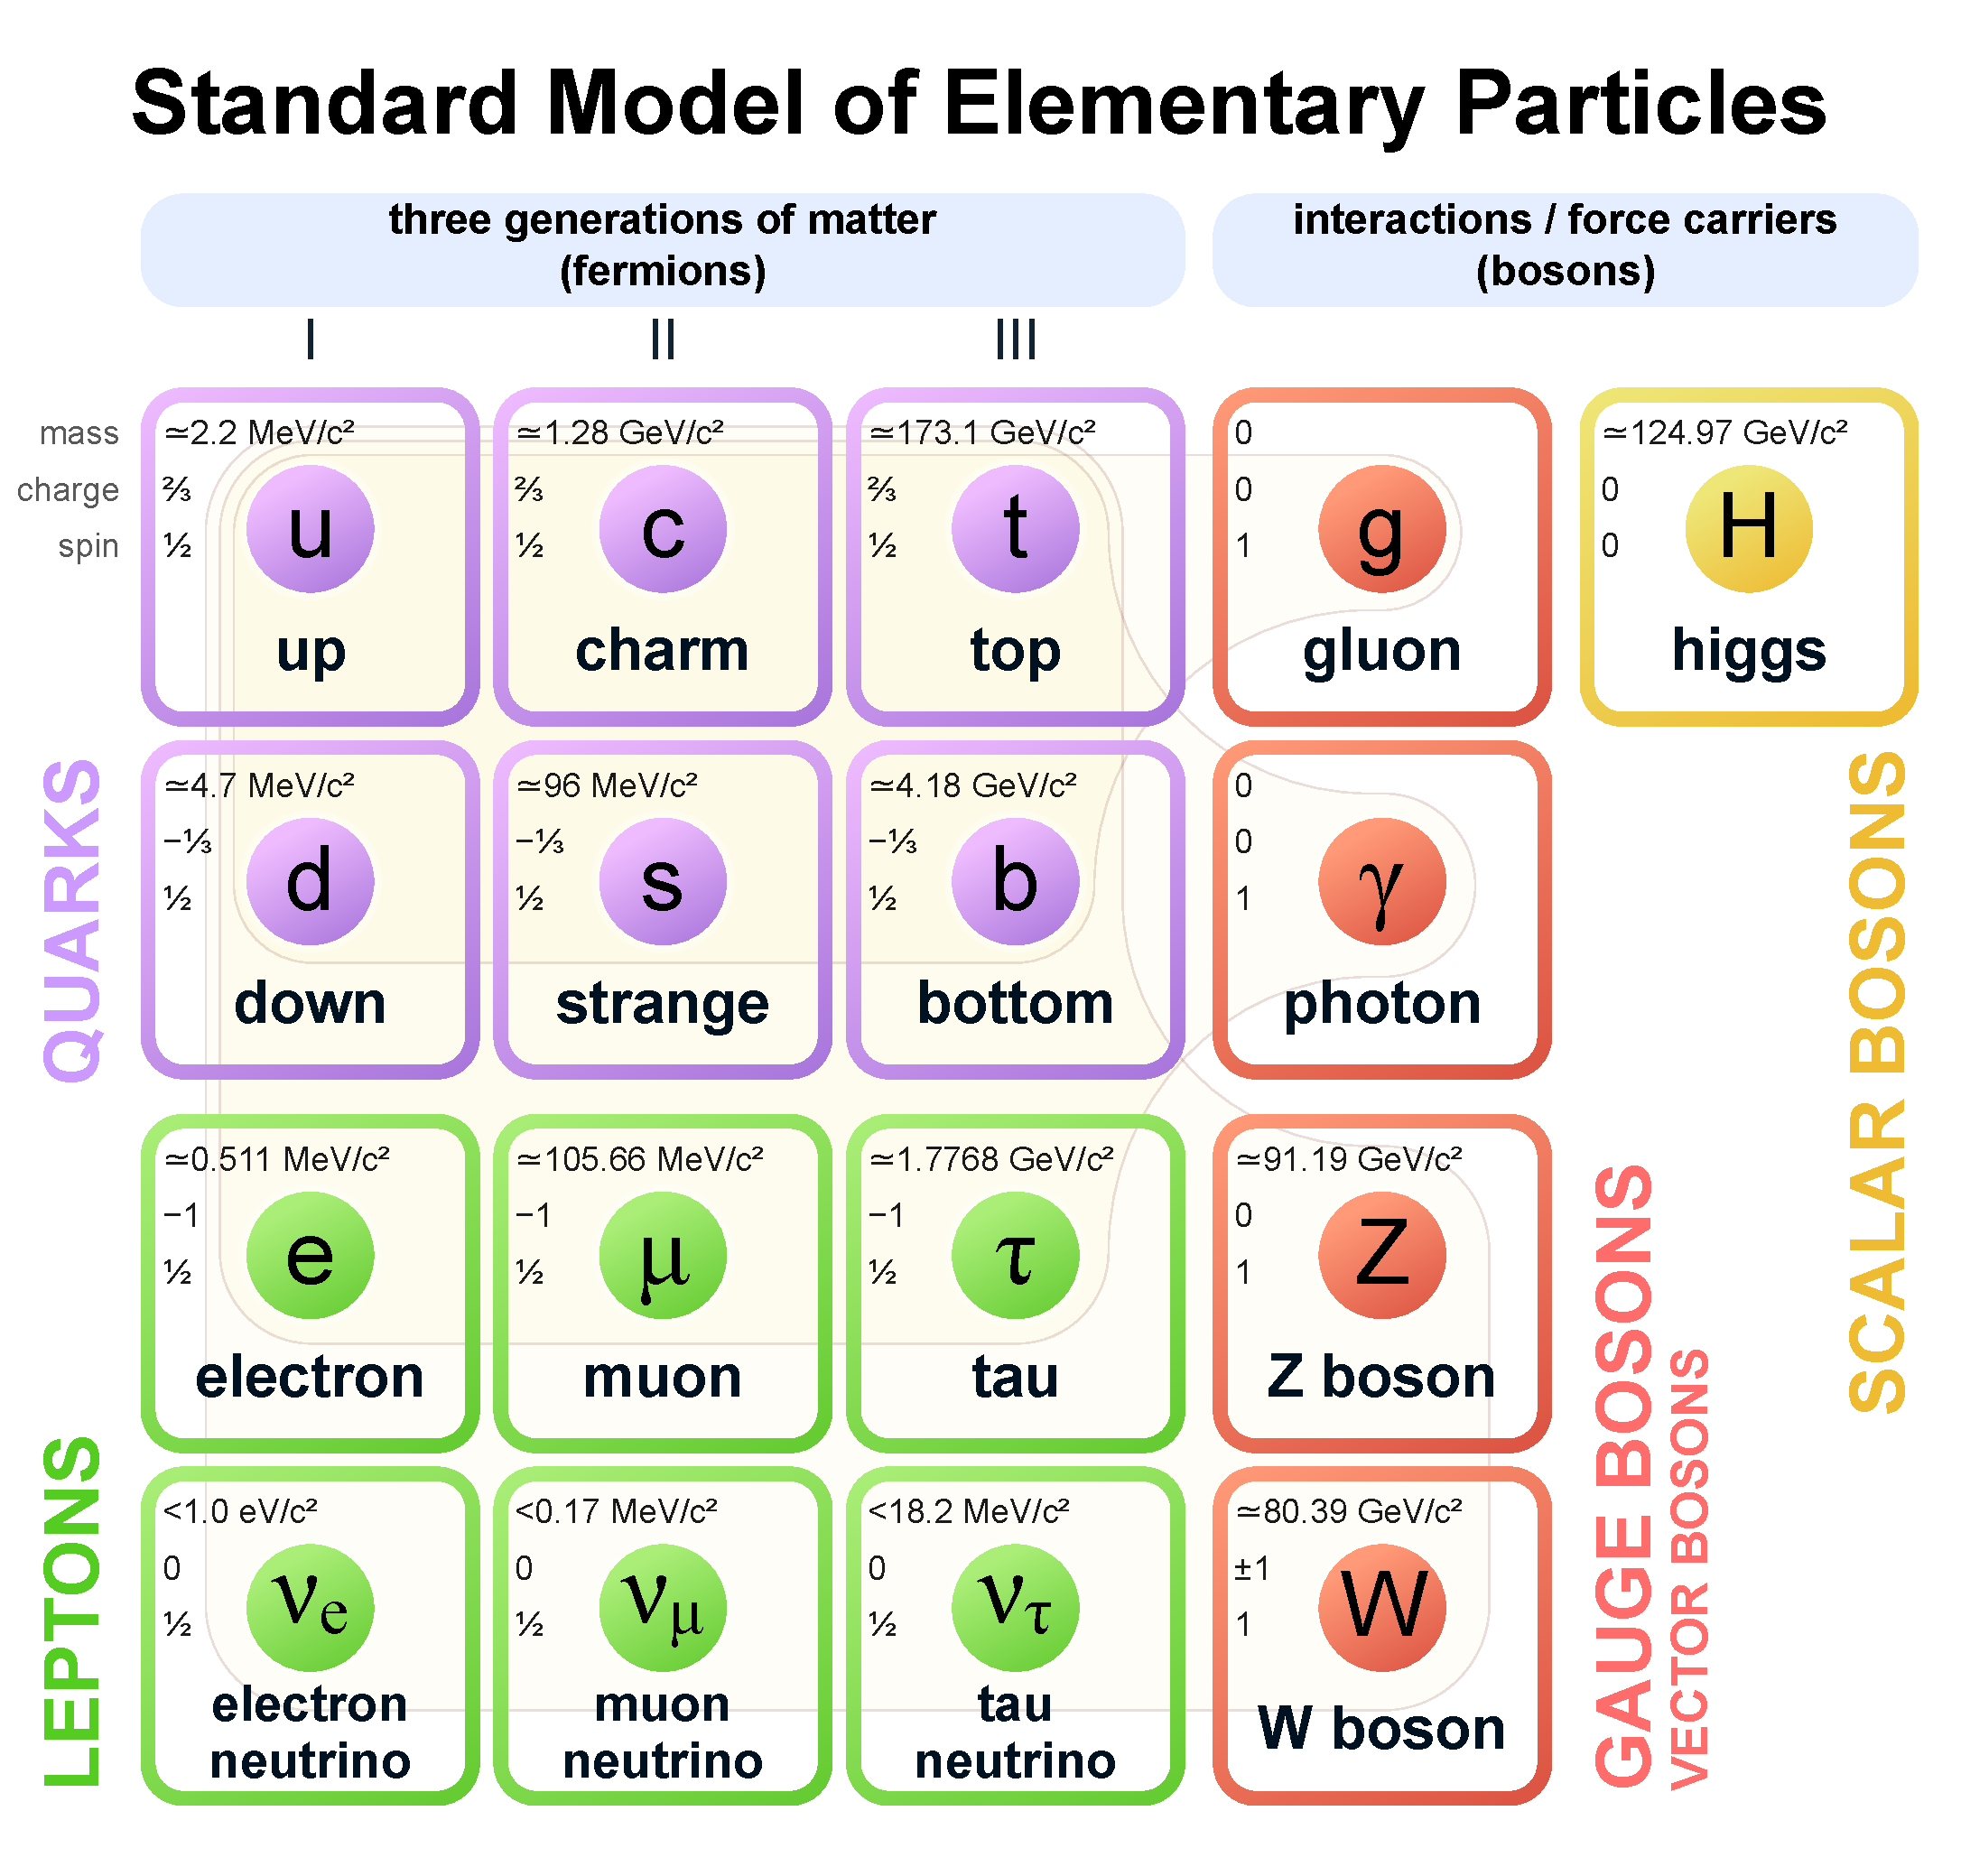
\includegraphics[width=0.7\textwidth]{figures/Theory/Standard_Model_of_Elementary_Particles.pdf}
  \caption{The elementary particles of the Standard Model.}
  \label{fig:eleP-1}
\end{figure}

\textbf{Fermions}
The Standard Model includes 12 elementary particles of spin-$\frac{1}{2}$ obeying the Fermy-Dirac statistics, known as fermions. 
They are classified into two types: \textit{leptons} and \textit{quarks} according to the their interactions.
The \textit{leptons} include three generations: electron ($e$) and electron neutrino ($\nu_{e}$); 
muon ($\mu$) and muon neutrino ($\nu_{\mu}$); tau ($\tau$) and tau neutrino ($\nu_{\tau}$).
The $e$, $\mu$ and $\tau$ carry electric charge of -1 and three neutrinos are electrically neutral. 
All the leptons can participate in electroweak interactions.
Also there are three generations of \textit{quarks}: up ($u$) and down ($d$); charm ($c$) and strange ($s$); top ($t$) and bottom ($b$).
The defining property of the quarks is that they carry color charge (while leptons don't), and hence interact via the strong interaction, 
letting them to be strongly bound from one to another, forming color-neutral composite 
particles (known as hadrons) containing either a quark and an antiquark (mesons) or three quarks (baryons).
In the meantime, $u$, $c$ and $t$ -quark carry electric charge of 2/3, and $d$, $s$ and $b$ -quark carry electric charge of -1/3. 
Hence they interact via all three interactions described in SM.
Each fermion also has its corresponding antiparticle.

\textbf{Gauge bosons}
act as force carriers that propagate the strong, weak, and electromagnetic interactions in SM.
They are spin-1 particles obeying the Bose-Einstein statistics. 
There are three types of gauge bosons:
\begin{itemize}
  \item The eight massless \textit{gluons} propagate the strong interactions between color charged particles (quarks).
  \item The massless \textit{photons} propagate the electromagnetic force between electrically charged particles.
  \item The $W^{+}$, $W^{-}$ and $Z$ bosons propagate the weak interactions between both quarks and leptons. All these three bosons are massive, the $W^{\pm}$ carries an electric charge of $+1$ and $−1$ and can also couple to the electromagnetic interaction while $Z$ boson is electrically neutral.
\end{itemize}
Figure~\ref{fig:eleP-2} shows the Feynman diagrams of corresponding interactions in SM.
\begin{figure}[!htb]
  \centering
  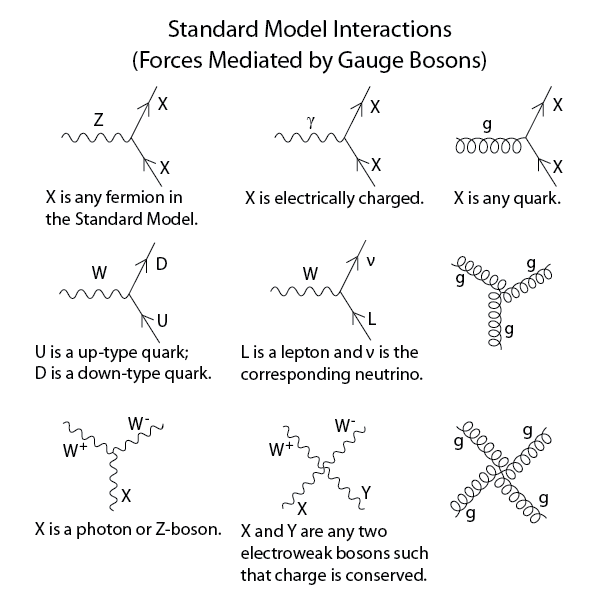
\includegraphics[width=0.8\textwidth]{figures/Theory/Standard_Model_Feynman_Diagram_Vertices.png}
  \caption{The Feynman diagrams of interactions mediated by gauge bosons that form the basis of the standard model.}
  \label{fig:eleP-2}
\end{figure}

\textbf{Higgs boson}
is a massive scaler elementary particle with spin-0. 
It plays a unique role in the SM by explaining the origin of masses of massive gauge bosons ($W^{\pm} and Z$) and fermions. 
And it is the last discovered particle in SM.

%\subsection{Elementary particles in the Standard Model}
\subsection{Electroweak theory}
\label{ewktheory}
The electroweak interaction is the unified description of two of the four known fundamental interactions of nature: electromagnetism and the weak interaction.
It is based on the gauge group of $SU(2)_{L} \times SU(1)_{Y}$, in which $L$ is the left-handed fields and $Y$ is the weak hypercharge \cite{Langacker:2009my}.
It follows the Lagrangian of
\begin{equation} \label{eq:Lew}
	L_{EW} = L_{gauge} + L_{Higgs} + L_{fermion} + L_{Yukawa}
\end{equation}

$L_{gauge}$ is the \textbf{gauge term} part
\begin{equation}
	L_{gauge} = -\frac{1}{4} W^{i}_{\mu\nu} W^{\mu\nu i} - \frac{1}{4} B_{\mu\nu} B^{\mu\nu}
\end{equation}
where $W^{i}_{\mu}$ and $B_{\mu}$ respectively present the $SU(2)_{L}$ and $SU(1)_{Y}$ gauge fields, with the corresponding field strength tensors of
\begin{equation}
\begin{split}
	& B_{\mu\nu} = \partial_{\mu} B_{\nu} - \partial_{\nu} B_{\mu} \\
	& W^{i}_{\mu\nu} = \partial_{\mu} W^{i}_{\nu} - \partial_{\nu} W^{i}_{\mu} - g \epsilon_{ijk} W^{j}_{\mu} W^{k}_{\nu}
\end{split}
\end{equation}
In the equations above, $g$ is the $SU(2)_{L}$ gauge coupling and $\epsilon_{ijk}$ is the totally antisymmetric tensor.
The gauge Lagrangian has three and four-point self interactions of $W^{i}$, which result in triple and quartic gauge boson couplings.

The second term of the Lagrangian is the \textbf{scaler part}:
\begin{equation} \label{eq:Lhiggs}
	{L}_{Higgs} = \left(D^{\mu}\phi\right)^{\dagger}D_{\mu}\phi - V(\phi)
\end{equation}
where $\phi = \binom{\phi^{+}}{\phi^{0}}$  is a complex Higgs scalar,
and $V(\phi)$ is the Higgs potential which is restricted into the form of 
\begin{equation} \label{eq:Vhiggs}
	V(\phi) = +\mu^{2}\phi^{\dagger}\phi + \lambda\left(\phi^{\dagger}\phi\right)^{2}
\end{equation}
due to the combination of $SU(2)_{L} \times SU(1)_{Y}$ invariance and renormalizability.
In Eq.~\ref{eq:Vhiggs}, $\mu$ is a mass-dependent parameter and $\lambda$ is the quartic Higgs scalar coupling, 
which represents a quartic self-interaction between the scalar fields.
When $\mu^{2} < 0$, there will be spontaneous symmetry breaking (more details in section~\ref{symbreaking}).
To maintain vacuum stability, $\lambda > 0$ is required.
And in Eq.~\ref{eq:Lhiggs}, the gauge covariant derivative is defined as
\begin{equation}
	D_{\mu}\phi = \left(\partial_{\mu} +ig\frac{\tau^{i}}{2}W_{\mu}^{i} + \frac{ig^{'}}{2}B_{\mu}\right)\phi
\end{equation}
in which $\tau^{i}$ represents the Pauli matrices, and $g'$ is the $U(1)_{Y}$ gauge coupling.
The square of the covariant derivative results in three and four-point interactions between the gauge and scalar fields.

The third term of the Lagrangian is the \textbf{fermion part}
\begin{equation} \label{eq:Lfermion}
\begin{split}
  	{L}_{fermion} = \sum_{m=1}^{F} & ( \bar{q}_{mL^{i}}^{0}\gamma_{\mu}D_{\mu}q_{mL}^{0} + \bar{l}_{mL^{i}}^{0}\gamma_{\mu}D_{\mu}l_{mL}^{0} + \bar{u}_{mR^{i}}^{0}\gamma_{\mu}D_{\mu}u_{mR}^{0} \\
  	& + \bar{d}_{mR^{i}}^{0}\gamma_{\mu}D_{\mu}d_{mR}^{0} + \bar{e}_{mR^{i}}^{0}\gamma_{\mu}D_{\mu}e_{mR}^{0} + \bar{\nu}_{mR^{i}}^{0}\gamma_{\mu}D_{\mu}\nu_{mR}^{0})
\end{split}
\end{equation} 
In Eq.~\ref{eq:Lfermion}, m is the family index of fermions, F is the number of families.
The subscripts $L (R)$ stand for the left (right) chiral projection $\psi_{L(R)} \equiv \left(1 \mp \gamma_{5} \right) \psi/2$.
\begin{equation}
	q_{mL}^{0} = \binom{u_{m}^{0}}{d_{m}^{0}}_{L}   \qquad    l_{mL}^{0} = \binom{\nu_{m}^{0}}{e_{m}^{-0}}_{L}
\end{equation}
are the $SU(2)$ doublets of left-hand quarks and leptons, while 
$u_{mR}^{0}$, $d_{mR}^{0}$, $e_{mR}^{-0}$ and $\nu_{mR}^{0}$ are the right-hand singlets.

The last term in Eq.~\ref{eq:Lew} is \textbf{Yukawa term}
\begin{equation}
\begin{split}
	{L}_{Yukawa} =& -\sum_{m,n=1}^{F} [\Gamma_{mn}^{u}\bar{q}_{mL}^{0}\widetilde{\phi}u_{nR}^{0} + \Gamma_{mn}^{d}\bar{q}_{mL}^{0}\phi d_{nR}^{0} \\
	& + \Gamma_{mn}^{e}\bar{l}_{mn}^{0}\phi e_{nR}^{0} + \Gamma_{mn}^{\nu}\bar{l}_{mL}^{0}\widetilde{\phi}\nu_{nR}^{0}]+h.c.
\end{split}
\end{equation}
the matrices $\Gamma_{mn}$ refer to the Yukawa couplings between single Higgs doublet ($\phi$) and the various flavors of quarks (m) and leptons (n).


%\subsection{Electroweak theory}
\subsection{Higgs mechanism and Electroweak symmetry breaking}
\label{symbreaking}

As shown in previous subsection, the Lagrangian $L_{gauge}$ does not involve any mass term due to the requirement of gauge invariance.
So all the W and B bosons should be massless. But experimental observations show that the gauge bosons are massive.
Therefore, the gauge invariance must be broken spontaneously.
The Higgs field is introduced to break the $SU(2)_{L} \times U(1)_{Y}$ symmetry and
guage bosons and fermions can interact with Higgs filed to acquire their masses.
And this specific process is named \textit{Higgs mechanism} in SM.

The Higgs field $\phi$ is a doublet and can be written in a Hermitian basis as
\begin{equation}
	\phi = \binom{\phi^{+}}{\phi^{0}} = \frac{1}{\sqrt{2}} \binom{\phi_{1} - i\phi_{2}}{\phi_{3} - i\phi_{4}}
\end{equation}
where $\phi_{i} = \phi_{i}^{+}$ stand for four Hermitian field. 
In this new basis, the Higgs potential in Eq.~\ref{eq:Vhiggs} can be expressed as:
\begin{equation}
	V(\phi) = \frac{1}{2}\mu^{2}\left(\sum_{i=1}^{4}\phi_{i}^{2}\right) + \frac{1}{4}\lambda\left(\sum_{i=1}^{4}\phi_{i}^{2}\right)^{2}
\end{equation}
To simplify the situation, the axis in this four-dimensional space can be choosen to satisfied
~$\left<0\left| \phi_{i} \right|0\right> = 0$ for $i = 1, 2, 4$, and $<0\left| \phi_{3} \right|0> = v$. Thus,
\begin{equation}
	V(\phi) \rightarrow V(v) = \frac{1}{2}\mu^{2}v^{2} + \frac{1}{4}\lambda v^{4}
\end{equation}
The minimization of this potential depends on the sign of $\mu^{2}$ as shown in figure~\ref{fig:C2_Higgs_potential}.
When $\mu^{2} > 0$ the minimum occurs at $v = 0$, namely the vacuum is empty space and $SU(2)_{L} \times U(1)_{Y}$ symmetry is unbroken.
In the case of $\mu^{2} < 0$, the $v = 0$ symmetric point is no longer stable and the minimum occurs at nonzero value of 
$v = \left( -\mu^{2}/\lambda\right)^{1/2}$ which breaks the $SU(2)_{L} \times U(1)_{Y}$ symmetry.
\begin{figure}[!htb]
  \centering
  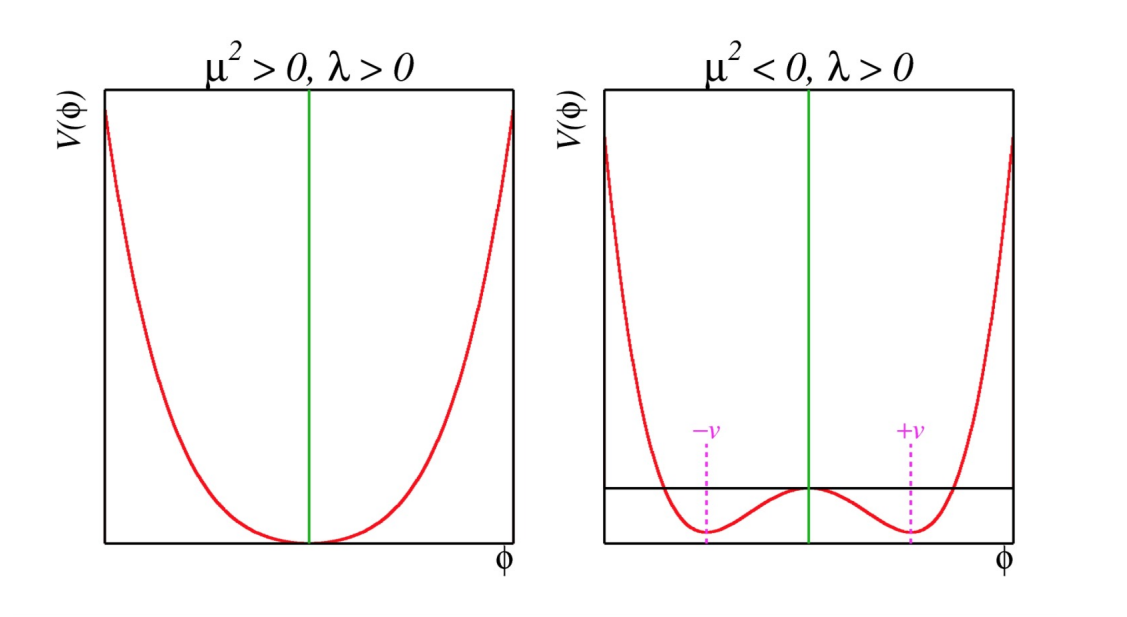
\includegraphics[width=0.7\textwidth]{figures/Theory/Vhiggs.png}
  \caption{Higgs potential $V(\phi)$ with $\mu^{2}>0$ (left) and $\mu^{2}<0$ (right).}
  \label{fig:C2_Higgs_potential}
\end{figure}
Thus, the classical vacuum $\phi_{0}$ of Higgs doublet can be expressed by
\begin{equation}
	\phi_{0} = \frac{1}{\sqrt{2}}\binom{0}{v}
\end{equation}
And to quantize around the classical vacuum in a general form:
\begin{equation}
	\phi = \frac{1}{\sqrt{2}} \binom{0}{v+H}
\end{equation}
Where H is a Hermitian field for physical Higgs scalar.
In this guage, the Lagrangian $L_{Higgs}$ in Eq.~\ref{eq:Lhiggs} takes a simple form
\begin{equation}
\begin{split} \label{eq:Lhiggs2}
	L_{Higgs} & = \left(D^{\mu}\phi\right)^{\dagger}D_{\mu}\phi - V(\phi) \\
	& = M_{W}^{2}W^{\mu+}W_{\mu}^{-}\left(1+\frac{H}{\nu}\right)^{2} + \frac{1}{2}M_{Z}^{2}Z^{\mu}Z_{\mu}\left(1+\frac{H}{\nu}\right)^{2} \\ 
        &   + \frac{1}{2}\left(\partial_{\mu}H\right)^{2} - V(\phi)
\end{split}
\end{equation}
where the W and Z fields are
\begin{equation}
\begin{split}
	& W^{\pm} = \frac{1}{\sqrt{2}} \left(W^{1} \mp iW^{2}\right) \\
	& Z = - sin\theta_{W}B + cos\theta_{W}W^{3}
\end{split}
\end{equation}
Therefore, in Eq.~\ref{eq:Lhiggs2} spontaneous symmetry breaking brings out masses for the W and Z gauge bosons
\begin{equation}
\begin{split}
	& M_{W} = \frac{gv}{2} \\
	& M_{Z} = \sqrt{g^{2} + g'^{2}} \frac{v}{2} = \frac{M_{W}}{cos\theta_{W}}
\end{split}
\end{equation}
where $\theta_{W}$ is the weak angle defined as
\begin{equation}
	sin\theta_{W} = \frac{g'}{\sqrt{g^{2} + g'^{2}}} \qquad cos\theta_{W} = \frac{g}{\sqrt{g^{2} + g'^{2}}} \qquad tan\theta_{W} = \frac{g'}{g}
\end{equation}
Then another gauge boson photon remains massless with the field of
\begin{equation}
	A = cos\theta_{W}B + sin\theta_{W}W^{3}
\end{equation}

After the symmetry breaking, the Higgs potential in unitary gauge can be written into
\begin{equation}
	V(\phi) = -\frac{\mu^{4}}{4\lambda} - \mu^{4}H^{2} + \lambda\nu H^{3} + \frac{\lambda}{4}H^{4}
\end{equation}
The first term in $V$ is a constant, while the second term denotes a (tree-level) mass of Higgs boson
\begin{equation}
	M_{H} = \sqrt{-2\mu^{2}} = \sqrt{2\lambda}v
\end{equation}
Due to the unknown of  quartic Higgs coupling $\lambda$, the Higgs mass is not predicted.
The third and fourth terms in Higgs potential $V$ denote the induced cubic and quartic interactions of the Higgs scalar.

Through the Higgs mechanism, fermions can also acquire their masses.
In the unitary gauge, Yukawa Lagrangian ($L_{Yukawa}$) can be written as a simple form of \cite{Pich:2015lkh}
\begin{equation}
	L_{Yukawa} = -\left(1+\frac{H}{v}\right) \left(m_{d}\bar{d}d + m_{u}\bar{u}u + m_{l}\bar{l}l\right)
\end{equation}
in which $m_{f} = \frac{y_{f}v}{\sqrt{2}}$ for $f = d, u, l$.

%\subsection{Higgs mechanics and electroweak symmetry breaking}

\section{Phenomenology of Large Hadron Collider}
The Large Hadron Collider (LHC) was built as a bridge between the theories and the experiment.
Physicists hope that the LHC can help to answer some of the fundamental open questions in physics, 
concerning the basic laws of interactions and forces among the elementary particles, 
the deep structure of space and time, and in particular the interrelation between quantum mechanics and general relativity.
This section will talk about firstly the general introduction of Physics inside hadronic collision,
then followed by two important LHC phenomenologies of the Higgs physics and Diboson physics that are related closely to this dissertation.

\subsection{Physics at hadronic collision}
\label{hadroniccollision}

Protons are not the elementery particle, which actually be composed of quarks and gluons.
So in proton-proton (pp) collision at LHC, it is not protons themselves interact but quarks and gluons.
Scattering processes can then be further classified into either \textit{hard} or \textit{soft} processes
according to the momentum transfer during the interaction \cite{Dremin:2005wd}.
QCD, as an underlying theory for both two process, its approach and level of understandings in two cases are quite different.
For hard process, eg. Higgs, vector bosons and jets production, the rates and event
properties can be precisely predicted based on perturbation theory.
However, for soft processes like total cross-section, the underlying events, the rates and properties are dominated by non-perturbative QCD effects
that are less understood.
For many hard processes, the hard interactions are accompanied by soft ones.
A example of the hadronic collision is illustrated in figure~\ref{fig:C2_had_col}. 
\begin{figure}[!htb]
  \centering
  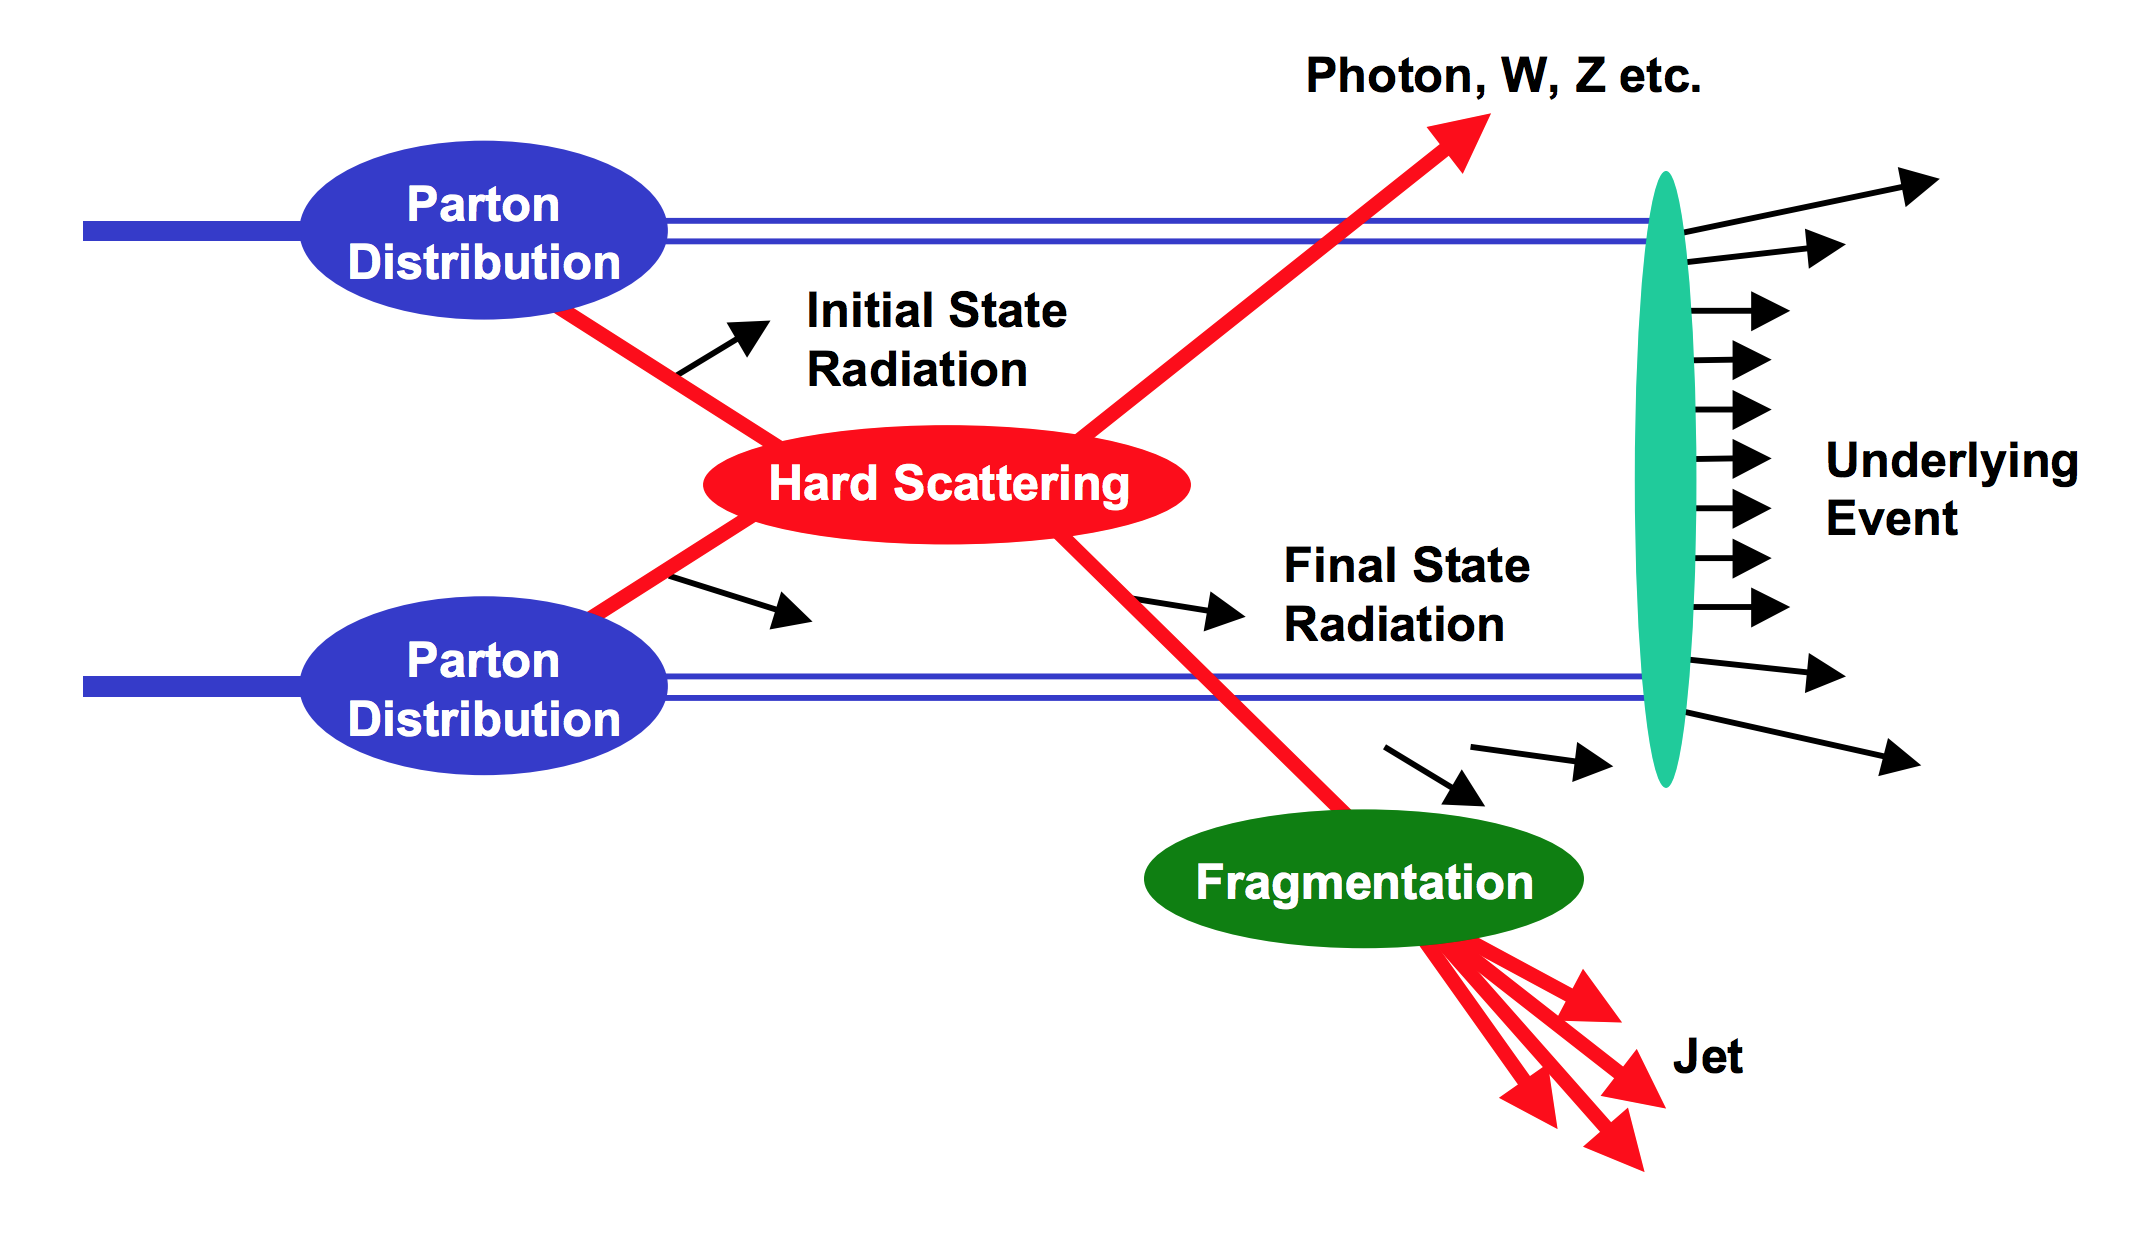
\includegraphics[width=0.7\textwidth]{figures/Theory/hh_collision.png}
  \caption{Schematic view of a hadron-hadron collision \cite{Womersley:2000cx}.}
  \label{fig:C2_had_col}
\end{figure}
and the typical features are summarized as below:
\begin{itemize}
	\item \textbf{Parton Distribution Function (PDF)} $f_{i}\left(x, Q^{2}\right)$ gives the probability of a parton with flavor $i$ (quark or gluon), carring amomentum fraction of $x$ and at the energy of Q in a proton. Parton distribution function cannot be fully calculated by perturbative QCD because of the inherent non-perturbative nature of partons. There are many different sets of PDFs that are determined by a fit to data from experimental observables in various processes. As an example, figure~\ref{fig:C2_PDF4LHC15} for \textit{PDF4LHC15} which is based on the combination of the \textit{CT14}, \textit{MMHT14} and \textit{NNPDF3.1} NNLO PDF sets \cite{Lin:2017snn}.
	\item \textbf{Fragmentation and hadronization} The processes to produce final state particles (or jets) from the partons produced in hard scattering.
	\item \textbf{Initial/Final state radiation} The incoming and outgoing partons that carry color charge can emit QCD radiation, which gives rise to additional jets. Also the charged incoming and outgoing particles can emit QED radiations with photons.
	\item \textbf{Underlying events} Products from soft processes (not come from the primary hard scattering) as the remnants of scattering interactions.
\end{itemize}
\begin{figure}[!htb]
  \centering
  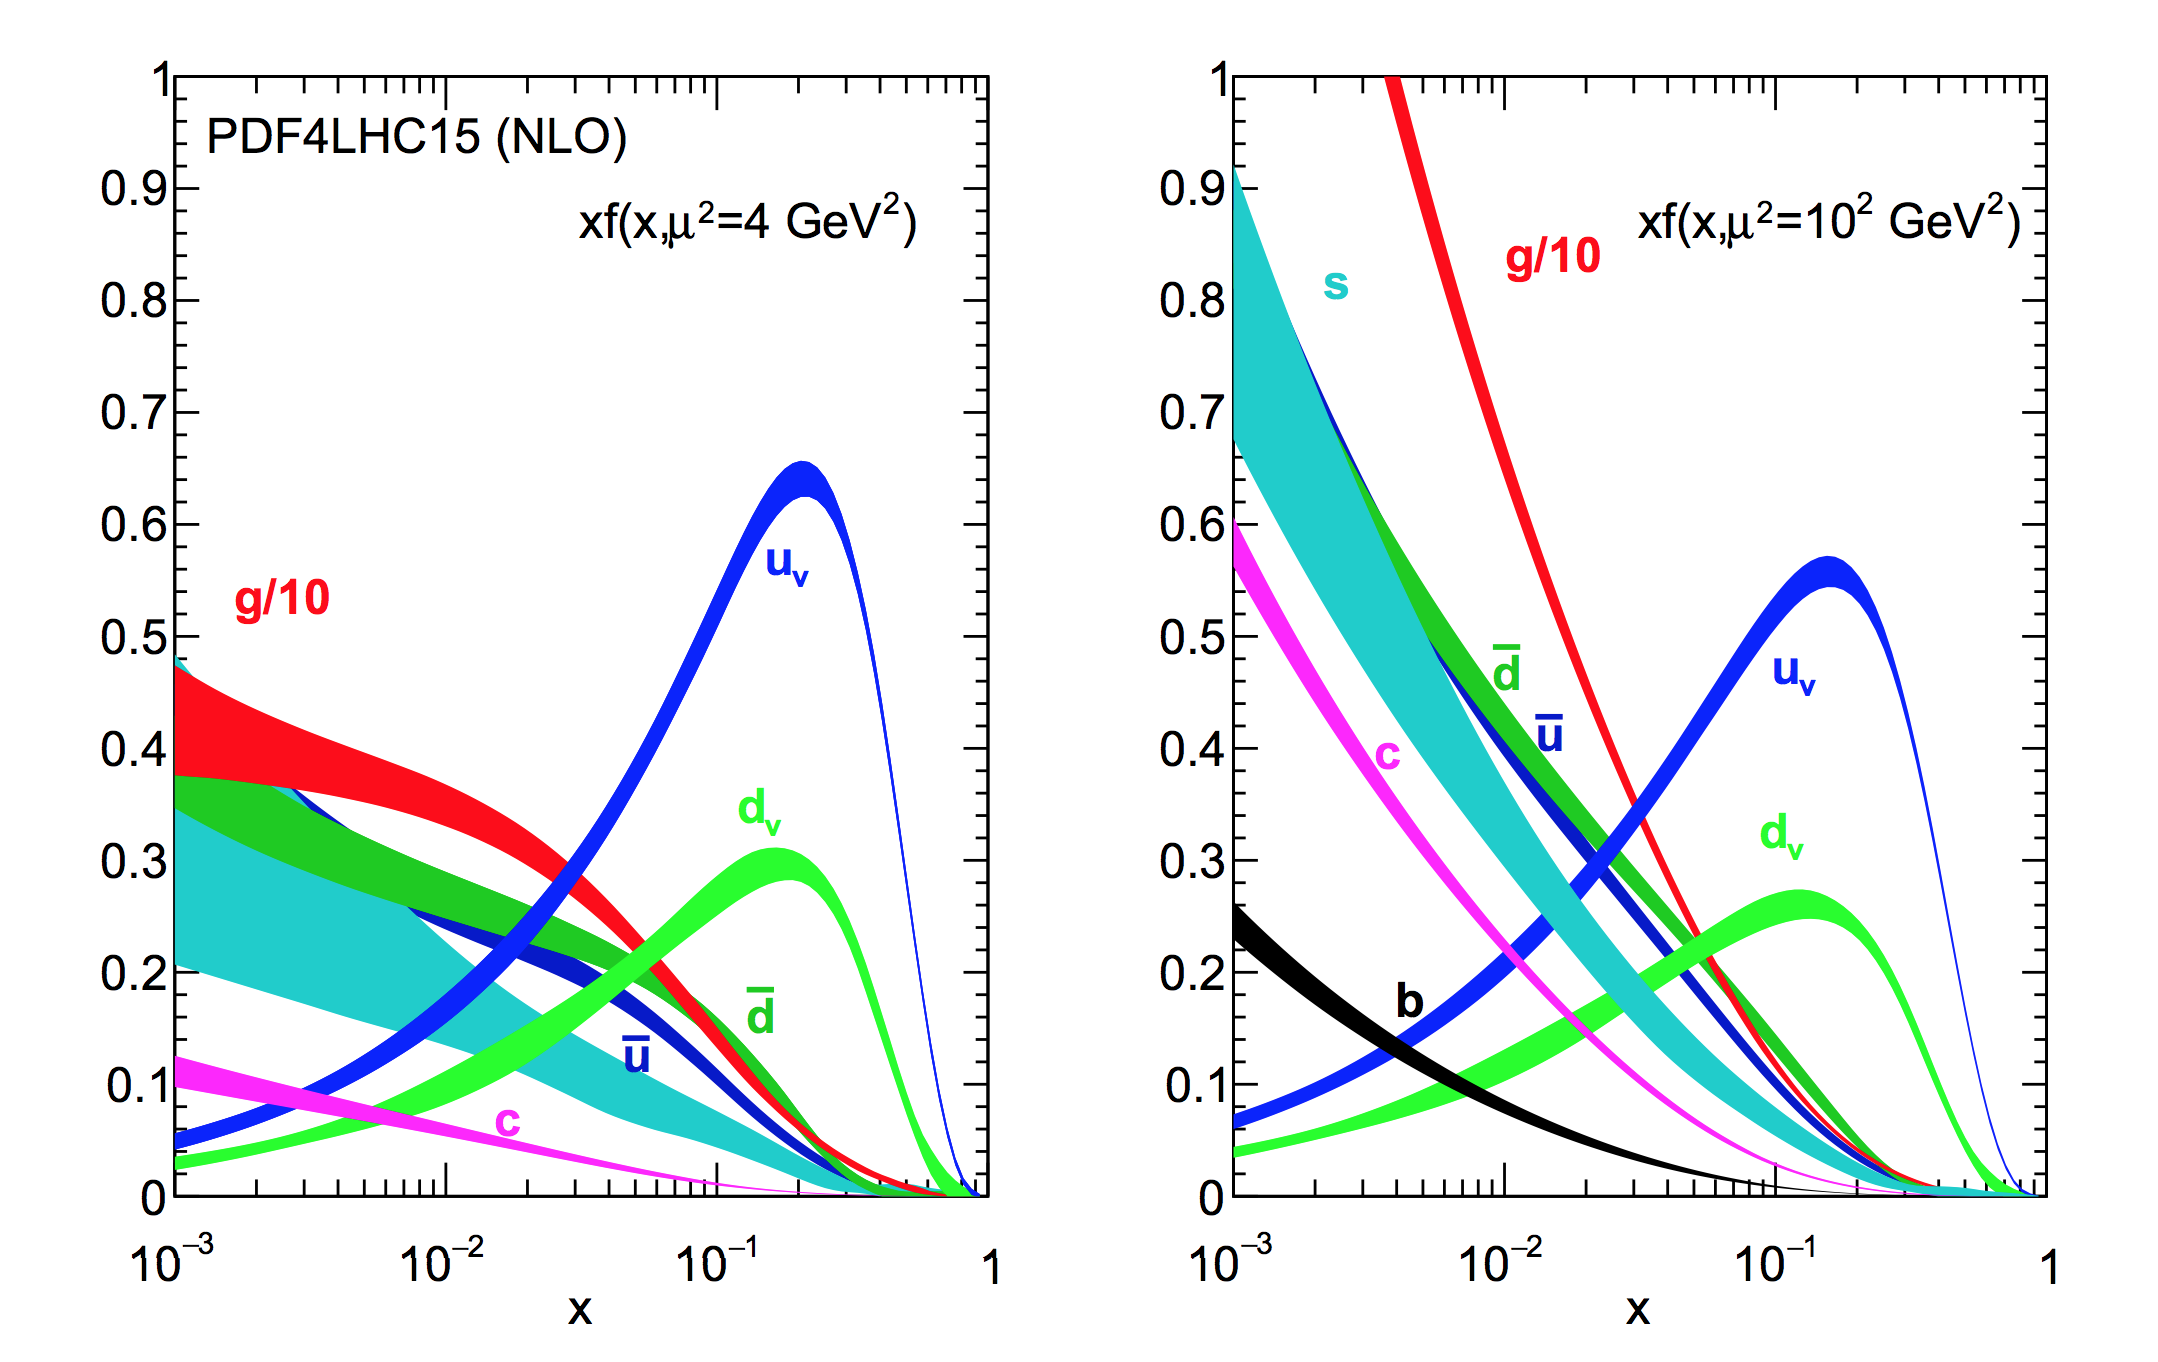
\includegraphics[width=0.7\textwidth]{figures/Theory/PDF4LHC15.png}
  \caption{The PDF4LHC15 NLO PDFs at a low scale $\mu^{2} = Q^{2} = 4 GeV^{2}$ (left) and at $\mu^{2} = Q^{2} = 100 GeV^{2}$ (right) as a function of x.}
  \label{fig:C2_PDF4LHC15}
\end{figure}

\textbf{Cross section of hard scaterring} 

According to \textit{QCD factorization theorems} \cite{Collins:1989gx}, the perturbative calculations can be applied to many important
hard processes involving hadrons. The basic problem addressed by factorization theorems is how to calculate high energy cross sections.
Conder the process of scattering between two hardons A and B to produce a final state X, the cross section $\sigma$ can be obtained 
by summing over all the subprocess cross section $\hat{\sigma}$ \cite{Stirling:1194745}
\begin{equation}
	\sigma_{AB} = \int dx_{a} dx_{b} f_{a/A}\left(x_{a}\right) f_{b/B}\left(x_{b}\right) \hat{\sigma}_{ab\rightarrow X}
\end{equation}
where $f_{q/A}\left(x_{q}\right)$ is the parton distrition functions of parton $q$.
Taking into account the leading order correction:
\begin{equation} \label{eq:xs2}
	\sigma_{AB} = \int dx_{a} dx_{b} f_{a/A}\left(x_{a}Q^{2}\right) f_{b/B}\left(x_{b}Q^{2}\right) \hat{\sigma}_{ab\rightarrow X}
\end{equation}
where $Q^{2}$ represents large momentum scale that characterizes the hard scattering.
Later on, since the finite corrections were not universal and had to be calculated separately for each process,
the perturbative $O\left(\alpha_{S}^{n}\right)$ corrections to the leading logarithm cross section in Eq.~\ref{eq:xs2}
need to be applied, one can get:
\begin{equation}
	\sigma_{AB} = \int dx_{a} dx_{b} f_{a/A}\left(x_{a}\mu_{F}^{2}\right) f_{b/B}\left(x_{b}\mu_{F}^{2}\right) \hat{\sigma}_{ab\rightarrow X}\left(\alpha_{S},\mu_{R},\mu_{F}\right)
\end{equation}
in which $\mu_{F}$ is \textit{factorization scale} which can represent the scale that separates the long- and short-distance physics,
and $\mu_{R}$ is the \textit{renormalization scale} for QCD running coupling.
$\hat{\sigma}_{ab\rightarrow X}$ is the parton-level hard scattering cross section that can be calculated perturbatively in QCD with the form of
\begin{equation} \label{eq:xs3}
	\hat{\sigma}_{ab\rightarrow X}\left(\alpha_{S},\mu_{R},\mu_{F}\right) 
		= \left(\alpha_{S}\right)^{n} \left[ \hat{\sigma}^{(0)}
		+ \left(\alpha_{S}/2\pi\right) \hat{\sigma}^{(1)}\left(\mu_{R},\mu_{F}\right)
		+ \left(\alpha_{S}/2\pi\right)^{2} \hat{\sigma}^{(2)}\left(\mu_{R},\mu_{F}\right)
		+ ... \right]
\end{equation}
where $\hat{\sigma}^{(0)}$ stands for the leading-order (LO) partonic cross section,
while $\hat{\sigma}^{(1)}$ and $\hat{\sigma}^{(2)}$ are the next-to-leading-order (NLO) and
next-to-next-to-leading-order (NNLO) cross section.

$\mu_{R}$ and $\mu_{F}$ depend on the order of truncation in Eq.~\ref{eq:xs3}.
In principle, if cross section is calculated to all orders, it is invariant under changes in these parameters.
The choices of $\mu_{R}$ and $\mu_{F}$ are arbitrary. 
To avoid unnaturally large logarithms reappearing in the perturbation series,
it is sensible to choose $\mu_{R}$ and $\mu_{F}$ values of the order of the typical momentum scales of
the hard scattering process and $\mu_{R} = \mu_{F}$ is also often assumed.
Take Drell–Yan process as an example, the standard choice is $\mu_{R} = \mu_{F} = m_{ll}$, 
where $m_{ll}$ is the invariant mass of dilepton pair.

%\subsection{Physics at hadronic collision}
\subsection{Higgs physics at LHC}
\label{higgs}

One important physics purpose of LHC is searching for Higgs boson, which was the last missing part in SM.
This section will talk about both the production and decay modes of SM Higgs boson in proton-proton collision.

%% ================================ Higgs production ===============================
\textbf{Higgs productions}

Higgs boson can be produced through several processes.
There are 4 main production modes at LHC: gluon-gluon fusion (\textit{ggF}), vector boson fusion (\textit{VBF}),
associated production with vector-bosons (also called Higgs strahlung) (\textit{VH}) 
and associated production with a pair of top/antitop quarks (\textit{ttH}) \cite{Grojean:2243593}.
Figure~\ref{fig:higgs_productions_fd} shows the corresponding Feynman diagrams of each process (at LO).
\begin{figure}[!htb]
  \centering
  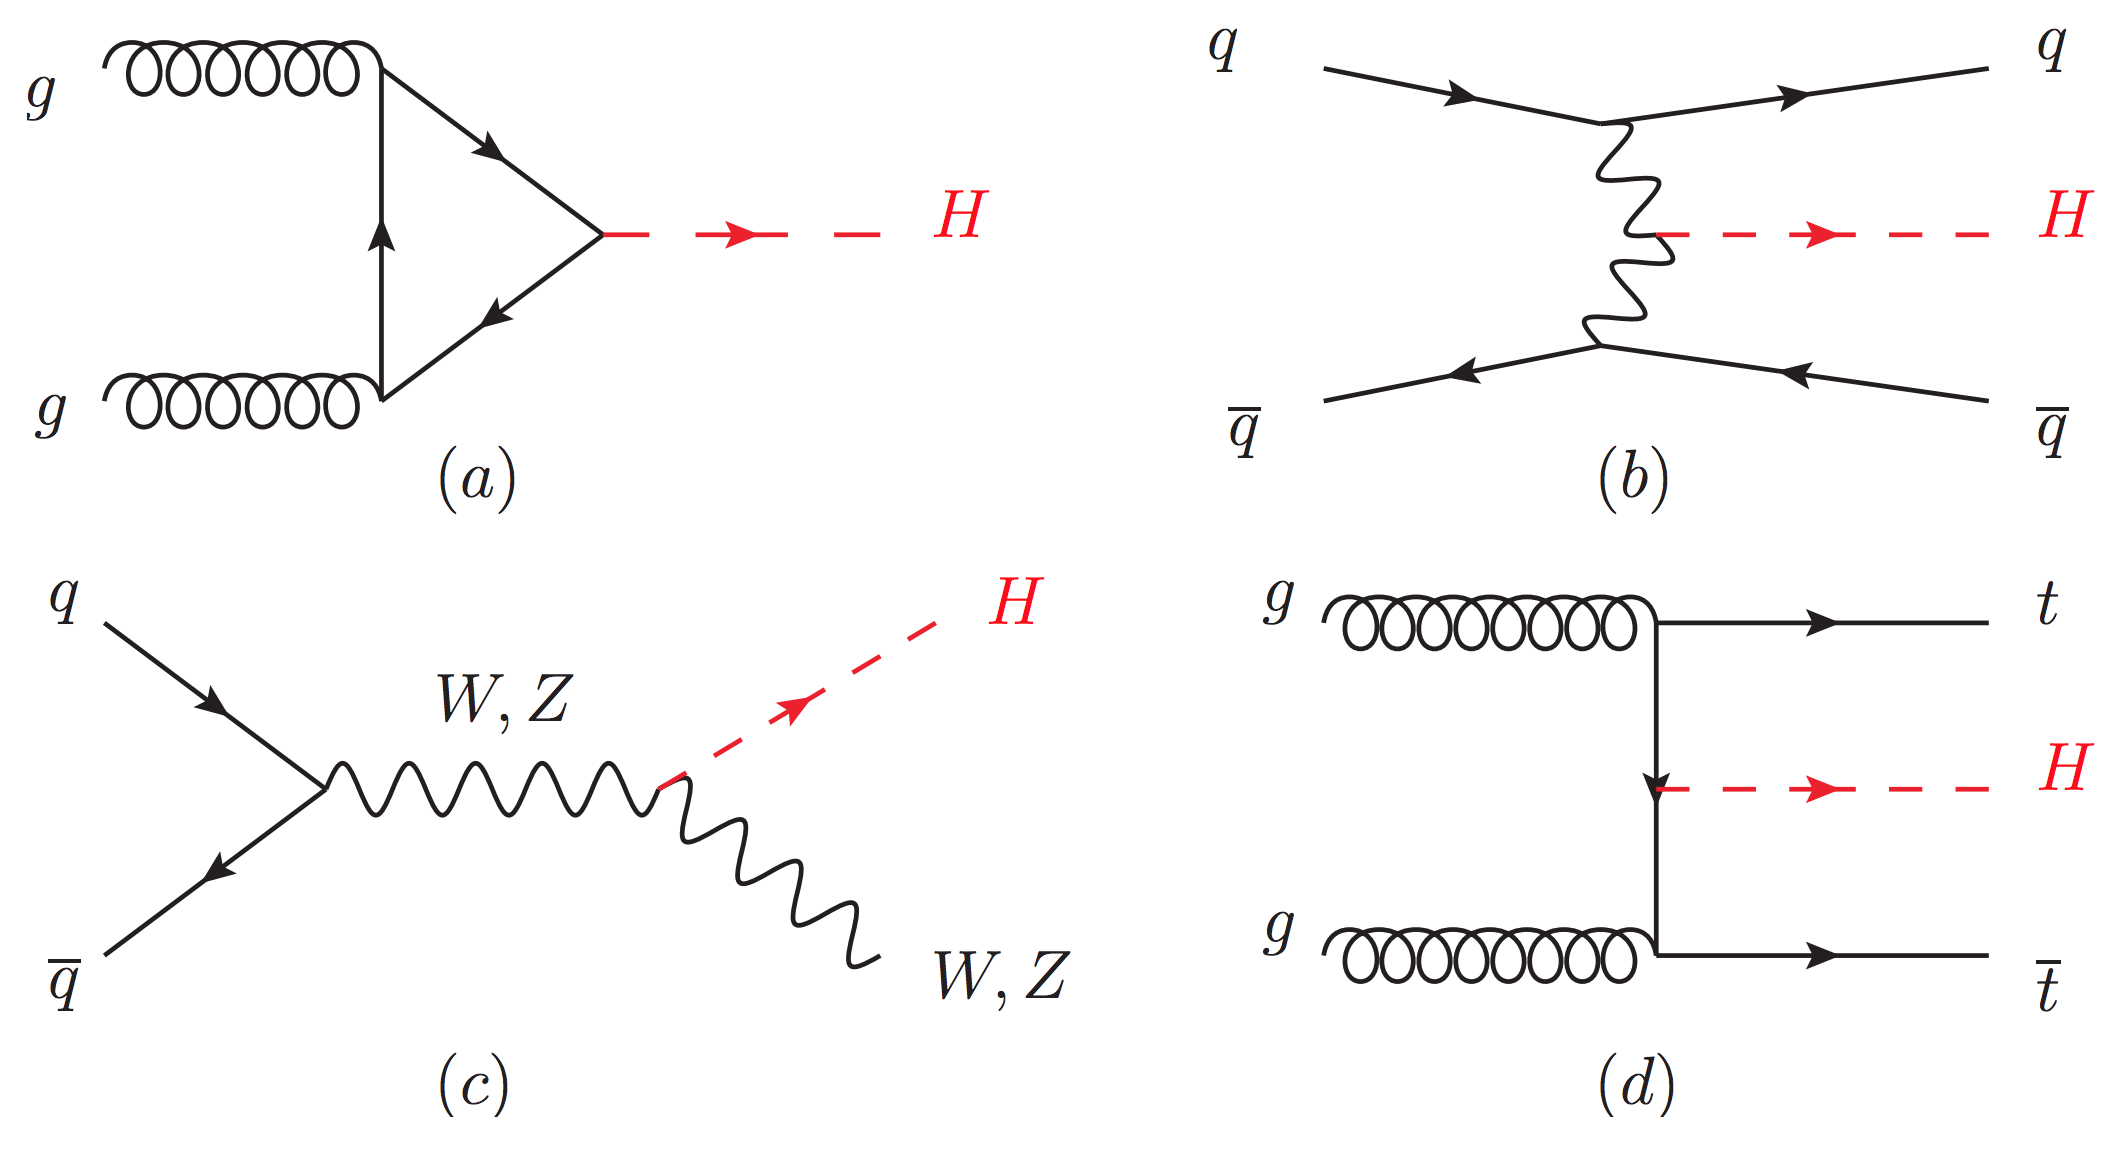
\includegraphics[width=0.8\textwidth]{figures/Theory/Figures_FeynmanHprod.png}
  \caption{Feynman diagrams of the Higgs production modes:
	   (a) ggF; (b) VBF; (c) VH; (d) ttH.}
  \label{fig:higgs_productions_fd}
\end{figure}
For pp collision, the cross section of productions of Higgs boson is as a function of center-of-mass-energy $\sqrt{s}$. 
Figure~\ref{fig:higgs_productions_xs} summarizes the cross section for SM Higgs with mass of 125 GeV.\\
\begin{figure}[!htb]
  \centering
  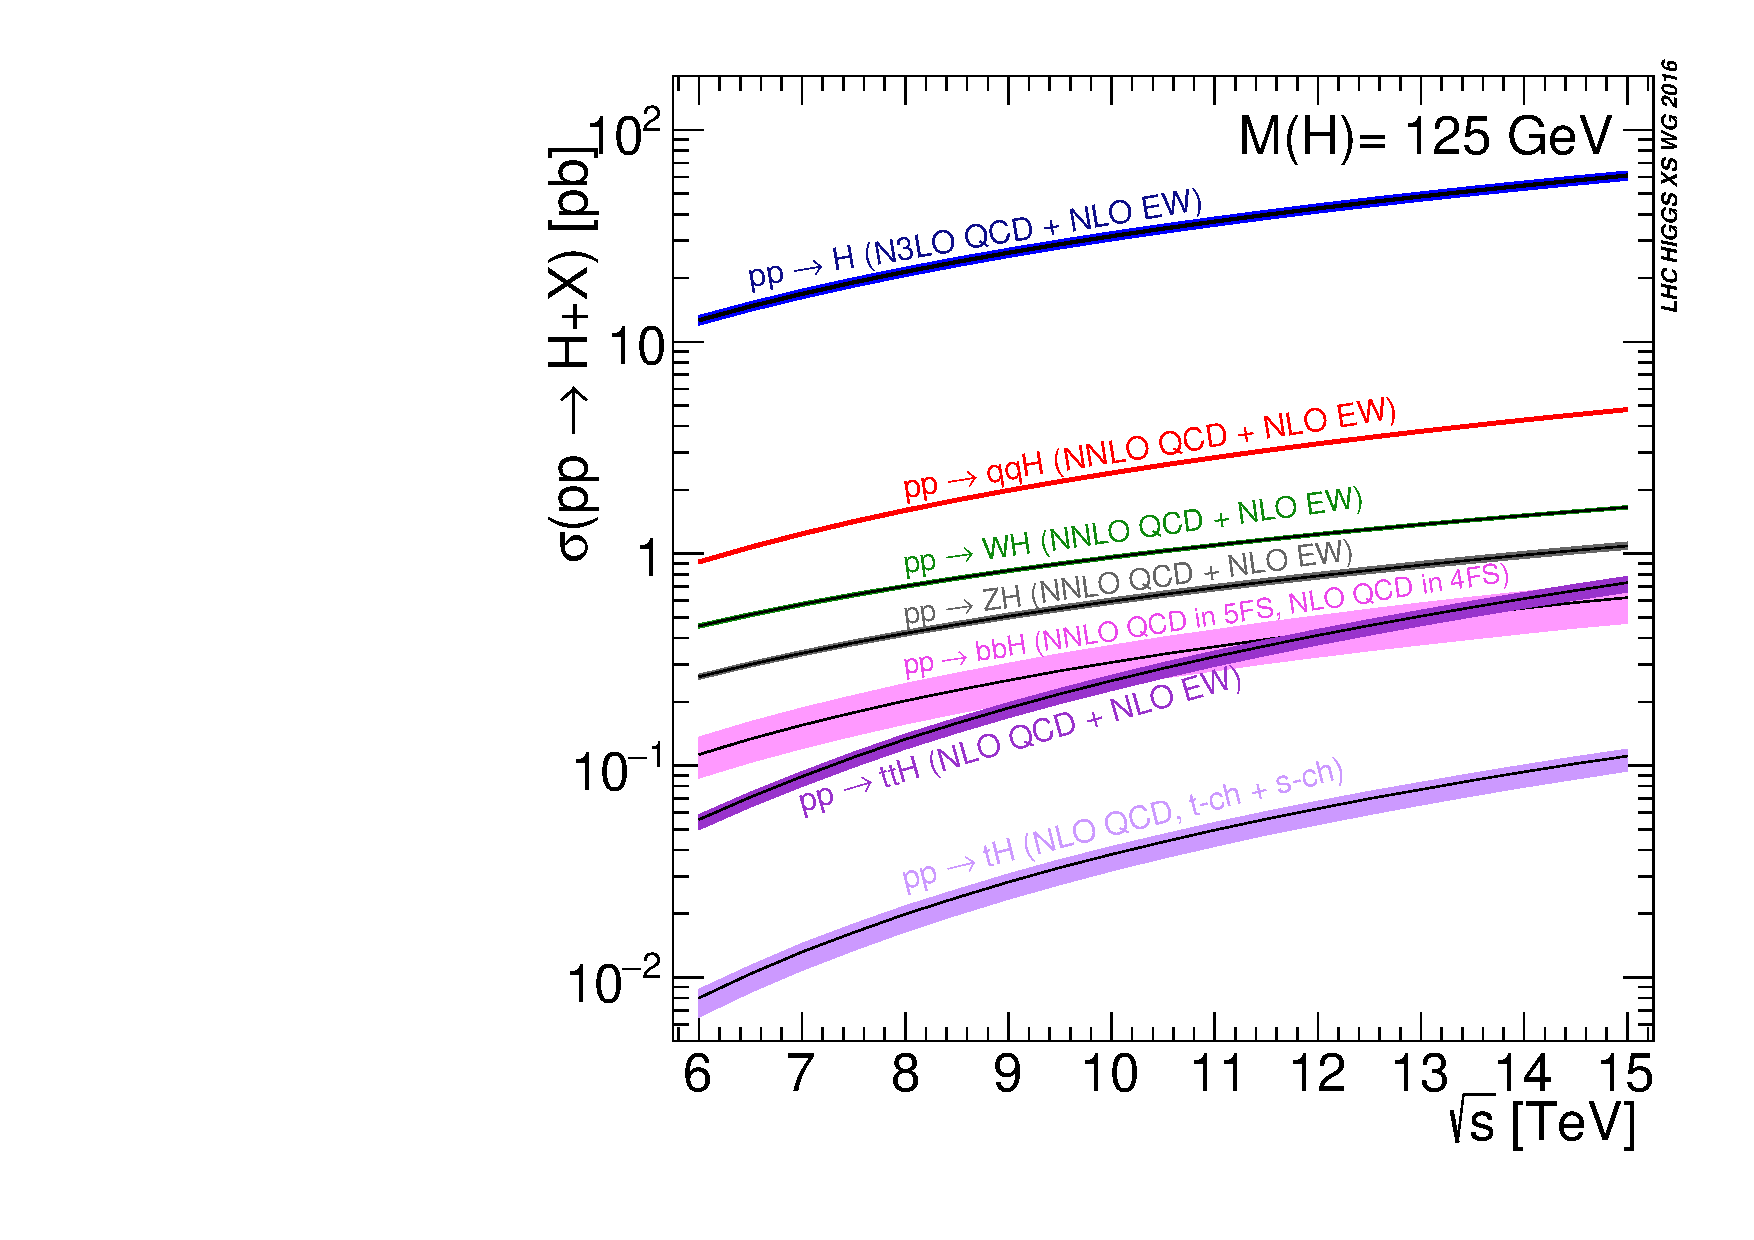
\includegraphics[width=0.5\textwidth]{figures/Theory/Plot_Escan_H125_new_sqrt.pdf}
  \caption{The SM Higgs boson production cross sections as a function of the center-of-mass-energy for pp collision.}
  \label{fig:higgs_productions_xs}
\end{figure}
Figure~\ref{fig:higgs_productions_xs2} summarizes the prospect of different Higgs boson production cross sections 
as a function of Higgs mass for pp collision center-of-mass-energy at 13 TeV and 14 TeV \cite{deFlorian:2227475}. 
\begin{figure}[!htb]
  \centering
  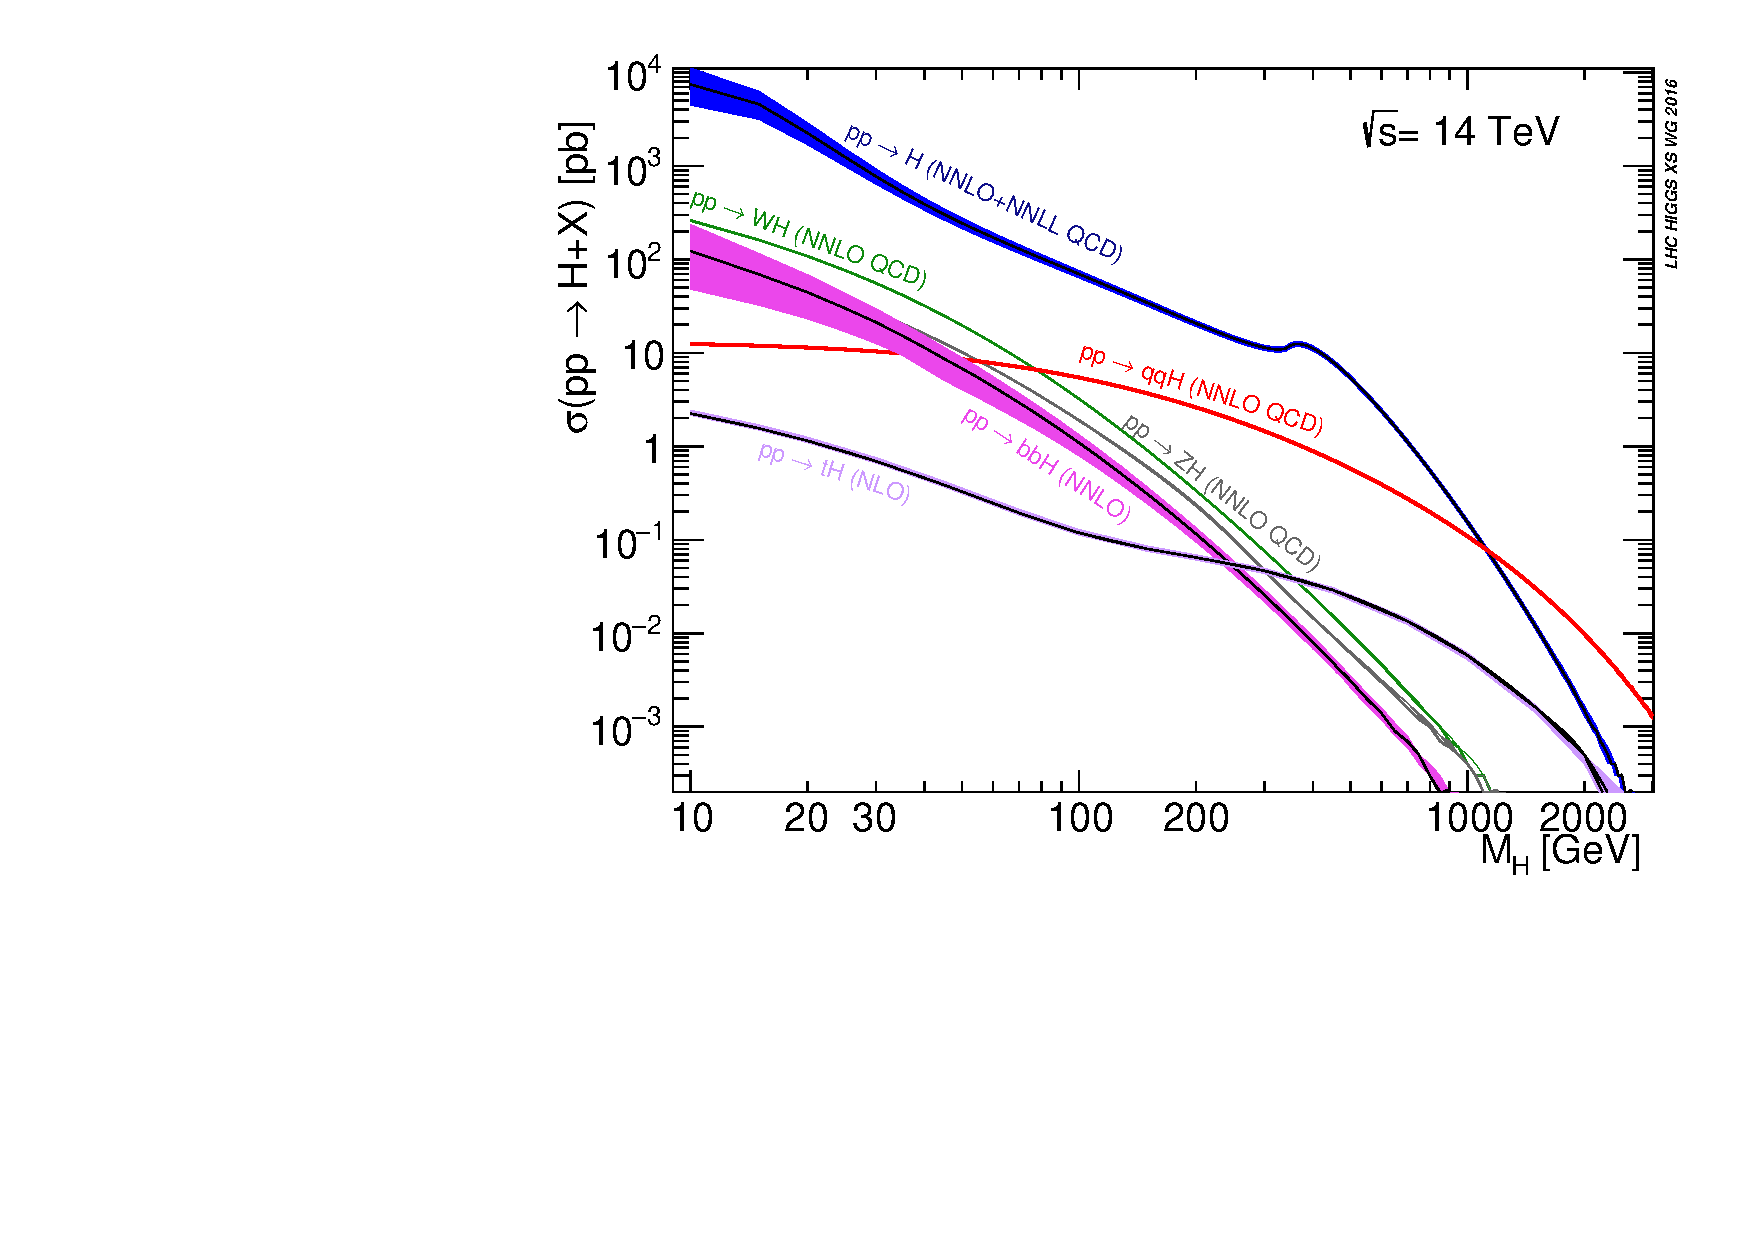
\includegraphics[width=0.45\textwidth]{figures/Theory/plotAll_14tev_BSM_sqrt.pdf}
  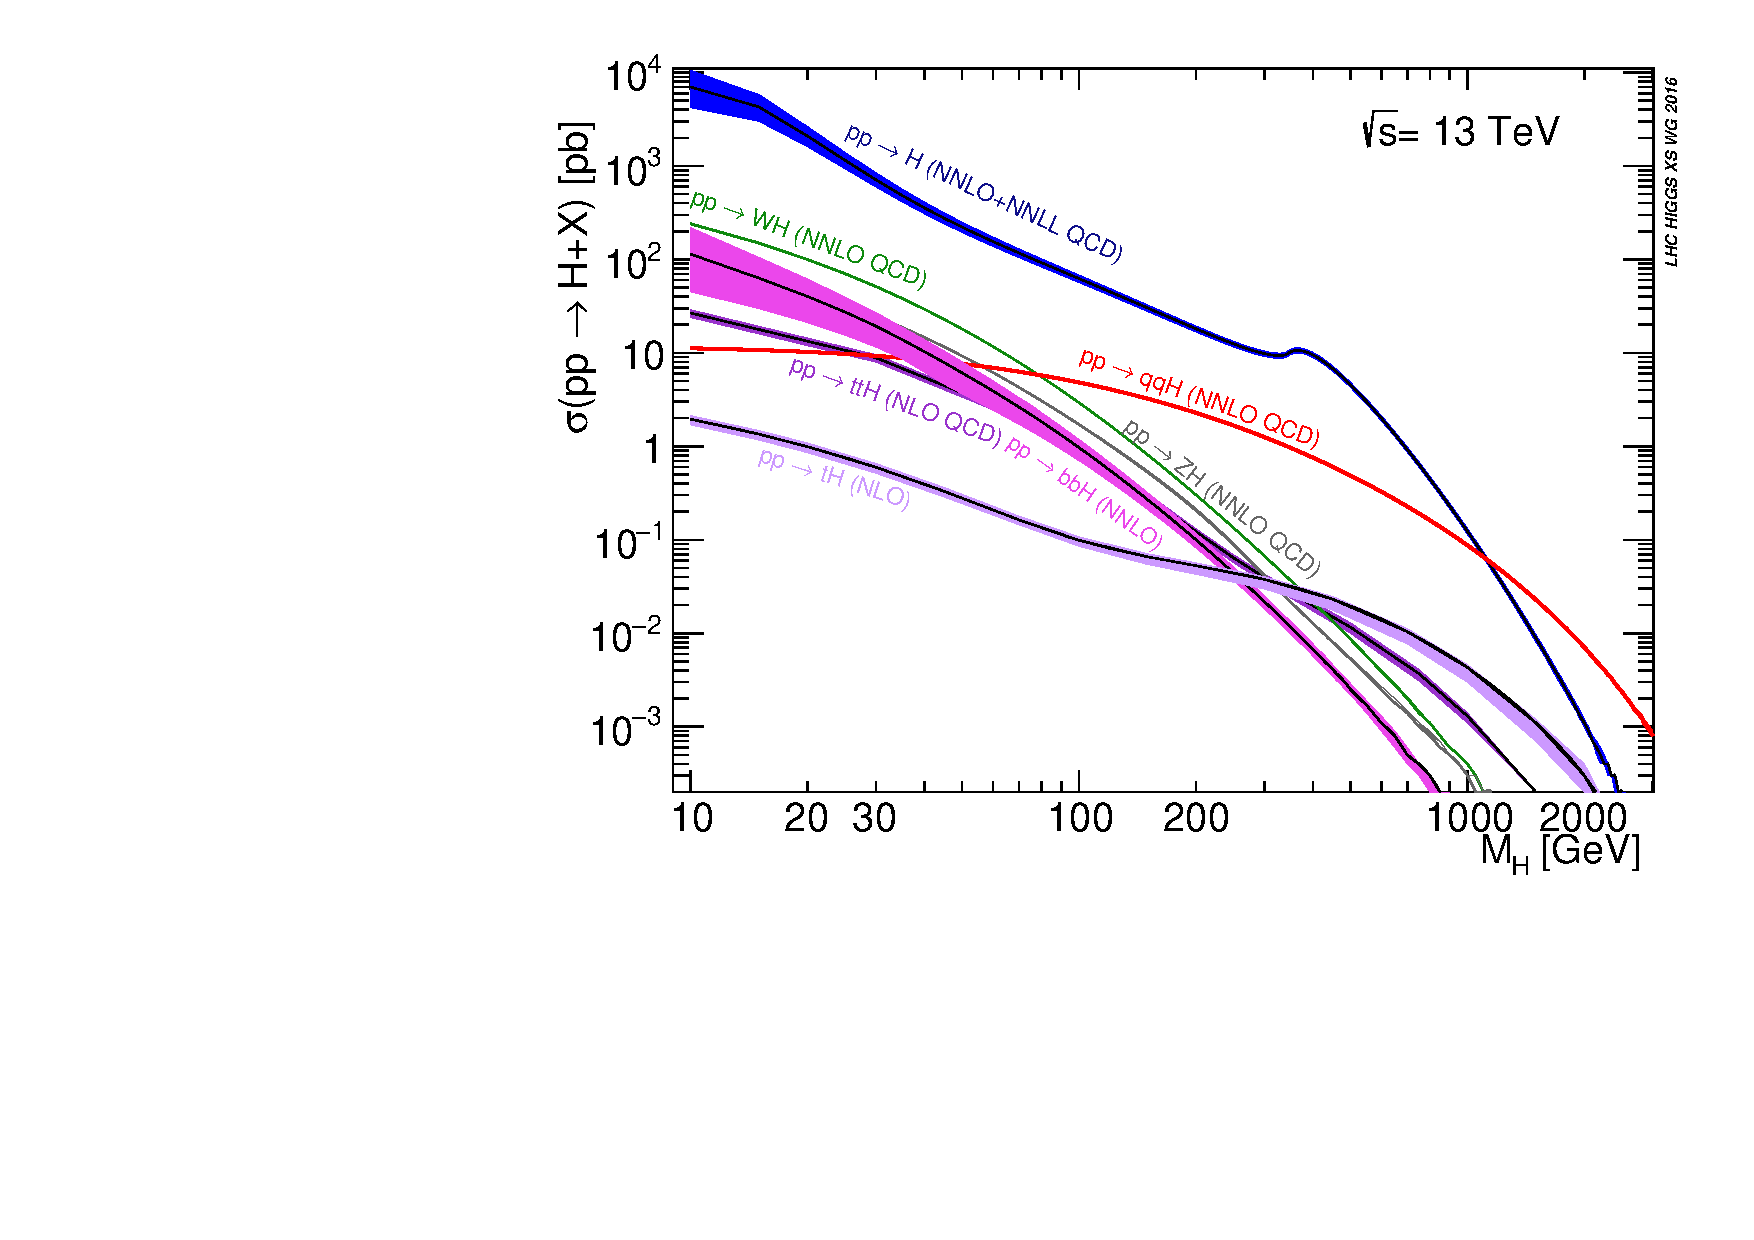
\includegraphics[width=0.45\textwidth]{figures/Theory/plotAll_13tev_BSM_sqrt.pdf}
  \caption{Higgs boson production cross section for various production modes as a function of the Higgs mass mH for $\sqrt{s}$ = 13 TeV (left) and 14 TeV (right) for pp collision.}
  \label{fig:higgs_productions_xs2}
\end{figure}

%% ================================ Higgs decays ===================================
\textbf{Higgs decays}

Higgs boson can interact with gauge bosons and fermions through gauge coupling and Yukawa coupling as introduced in section~\ref{symbreaking}.
Figure~\ref{fig:higgs_decay_fd} depicts Feynman diagrams of possible Higgs decay channels.
\begin{figure}[!htb]
  \centering
  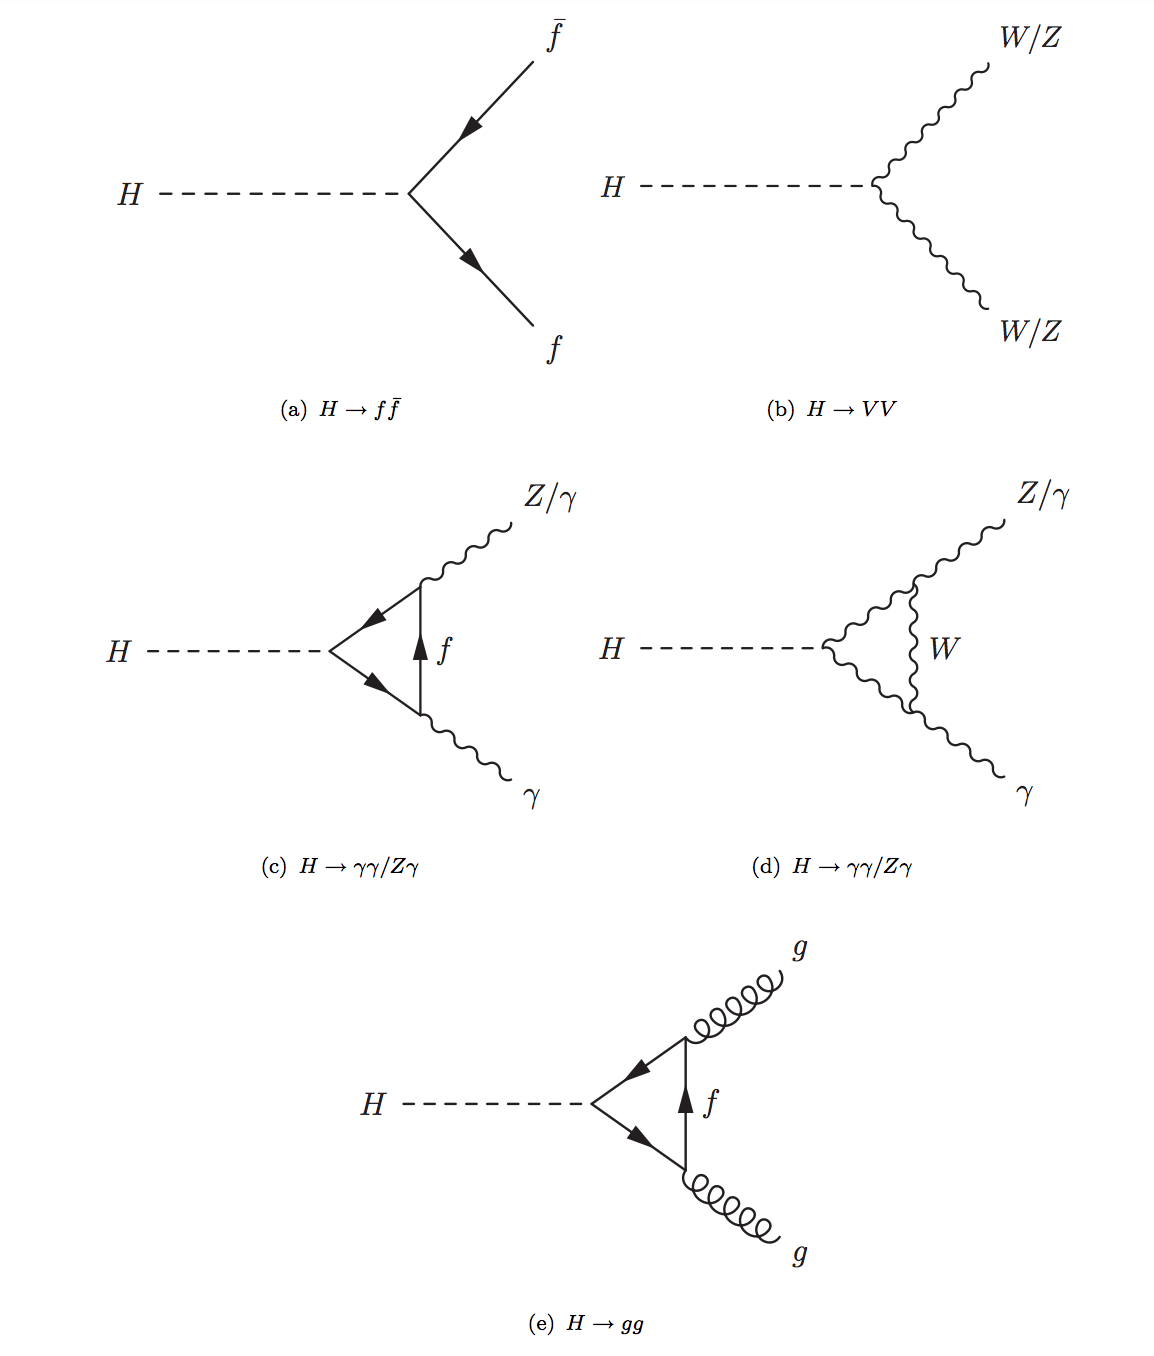
\includegraphics[width=0.8\textwidth]{figures/Theory/Figures_Feynman_Hdecay.png}
  \caption{SM Higgs decay channels.}
  \label{fig:higgs_decay_fd}
\end{figure}
The branching ratio of Higgs boson decaying into different final states as a function of Higgs mass is shown in figure~\ref{fig:higgs_decay_br}.
\begin{figure}[!htb]
  \centering
  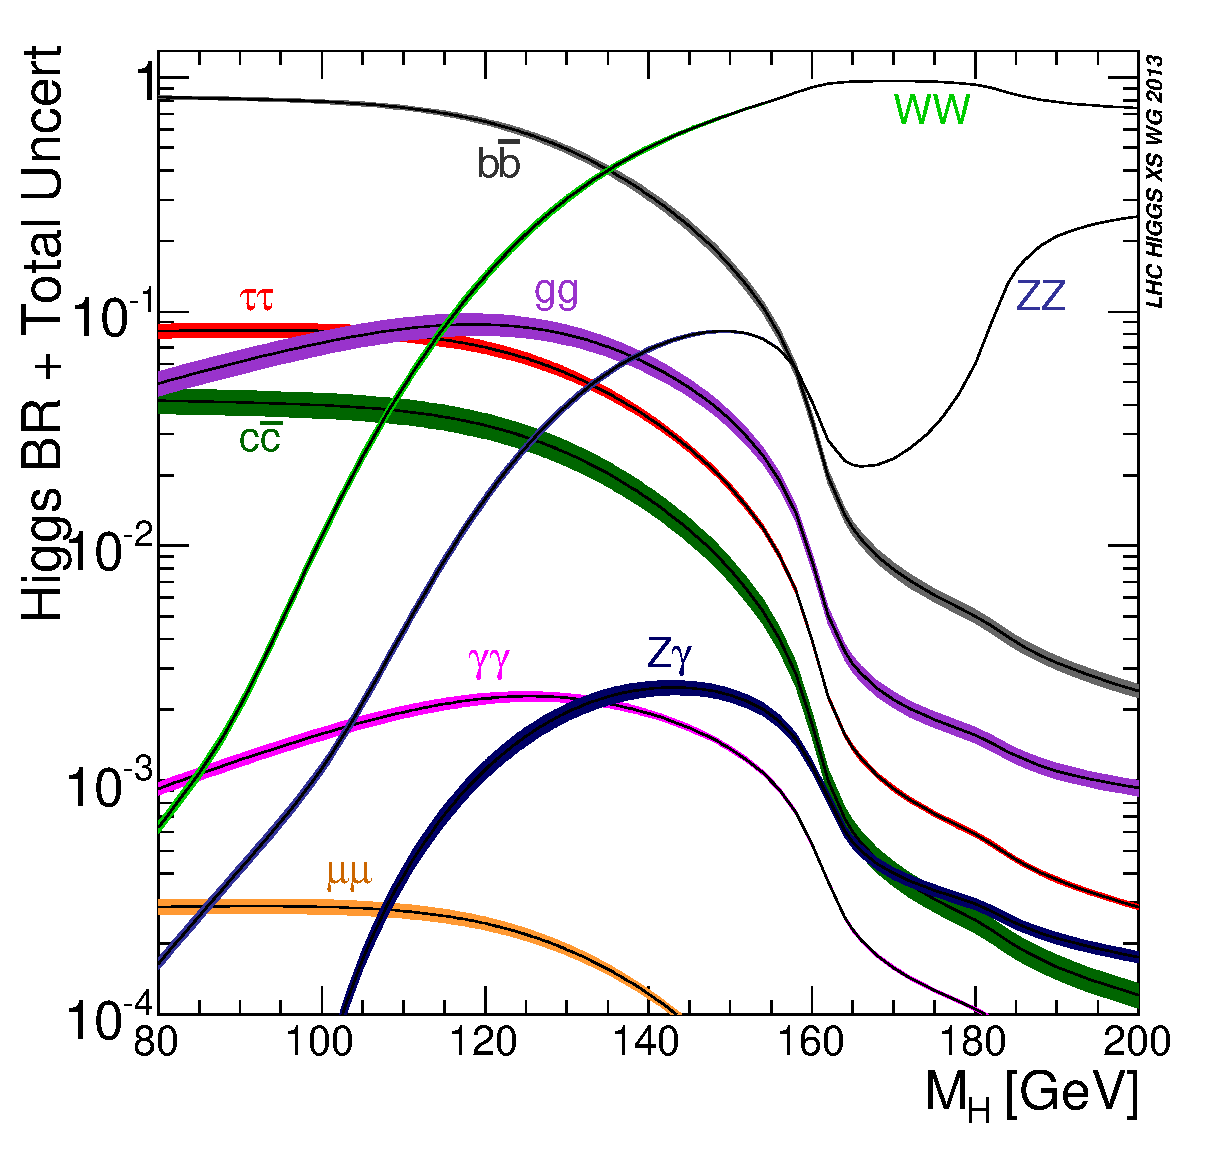
\includegraphics[width=0.5\textwidth]{figures/Theory/Higgs_BR_LM.eps}
  \caption{Branching ratio of Higgs decays \cite{Heinemeyer:1559921}. }
  \label{fig:higgs_decay_br}
\end{figure} 

%% ====================================== High mass related ===========================
(\textbf{BSM Higgs models})



%\subsection{Higgs Physics at LHC}
\subsection{Diboson physics}
\label{diboson}

The study of diboson physics is another important test for SM of particle physics in electroweak sector, 
in which vector boson scattering is a key process for probing the mechanism of electroweak symmetry breaking (EWSB).
In the meantime, the non-resonant diboson productions are crucial backgrounds for Higgs study at LHC, which make the precise measurement of their cross section becomes very important.

%% ====================================== Diboson productions ========================
\textbf{Diboson productions}

About $90\%$ of diboson productions at hadron collider is from quark-antiquark annihilation,
while others are contributed from gluon initiated process.
Figure~\ref{fig:diboson_fd1} shows the tree-level Feynman diagrams of diboson production.
\begin{figure}[!htb]
  \centering
  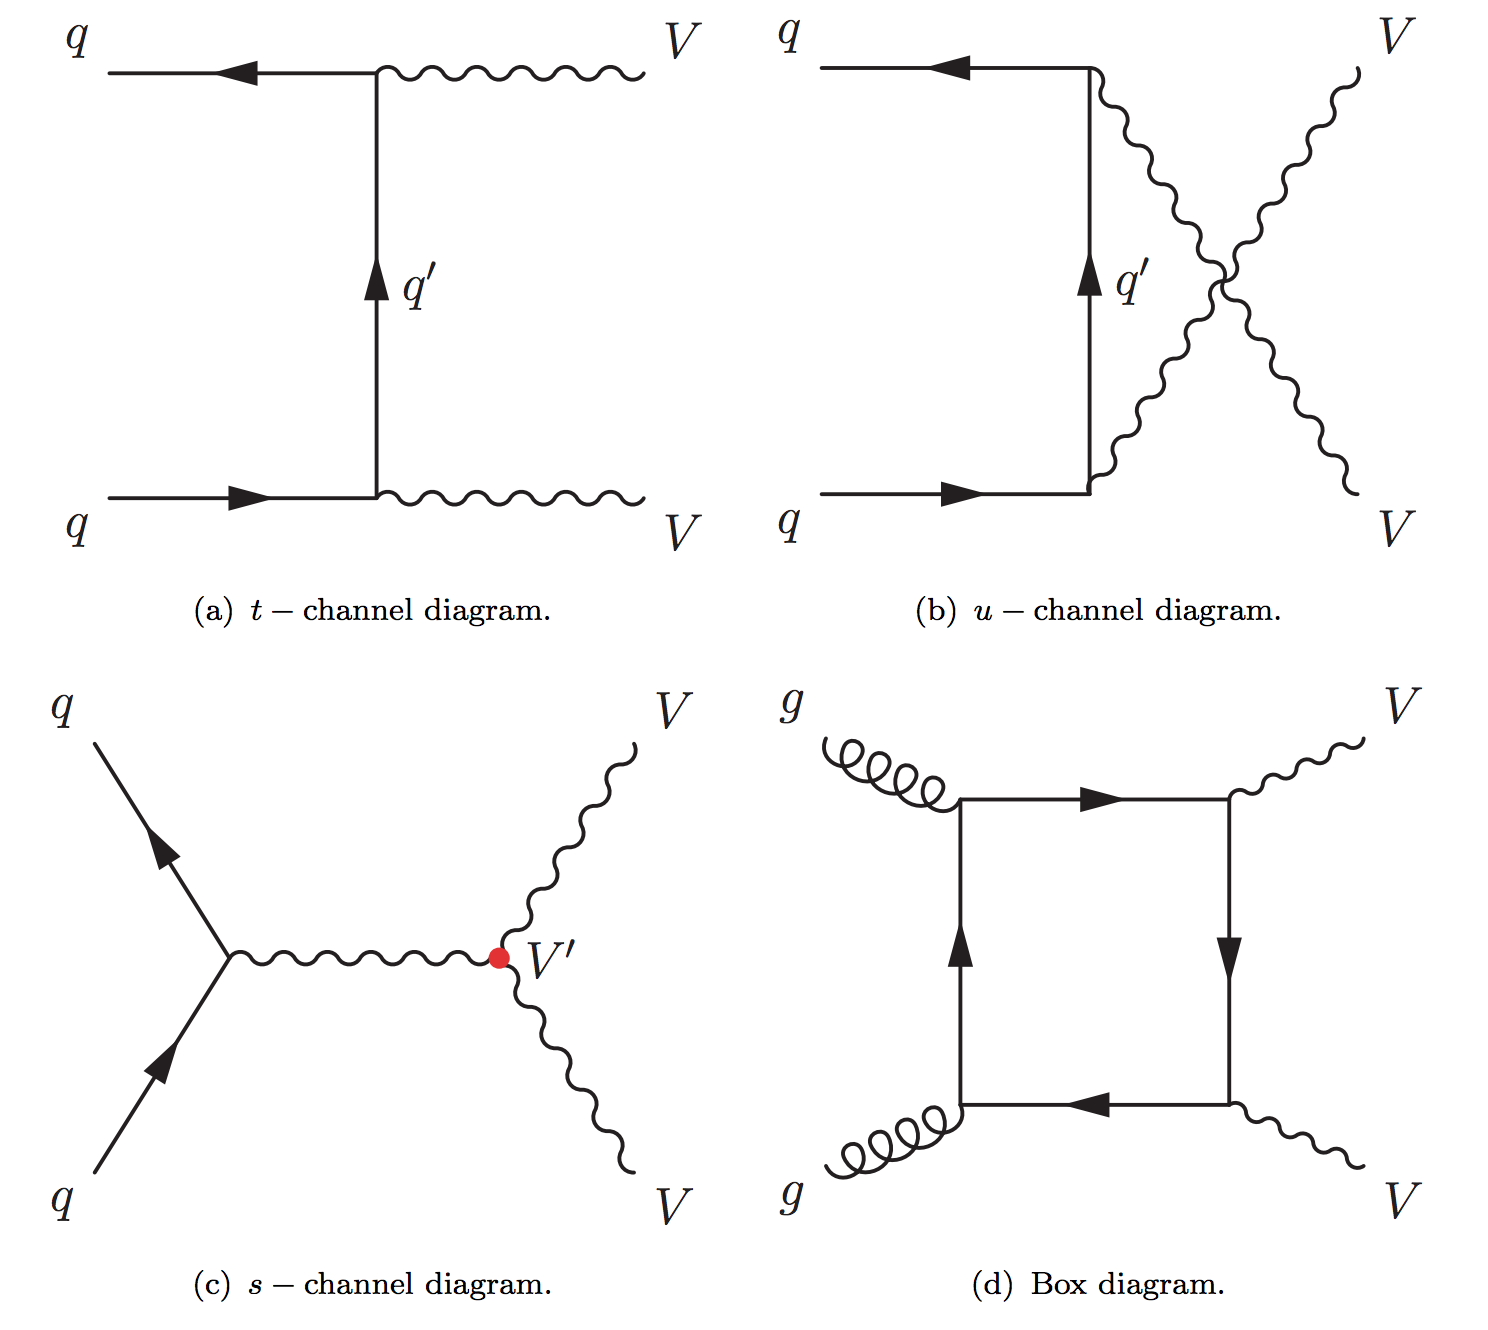
\includegraphics[width=0.7\textwidth]{figures/Theory/diboson_prod_fey.png}
  \caption{The tree-level Feynman diagrams of diboson production at LHC.}
  \label{fig:diboson_fd1}
\end{figure}
Then figure~\ref{fig:diboson_xs1} illuminates the total production cross-section presented by ATLAS
as a function of centre-of-mass energy $\sqrt{s}$ from 7 to 13 TeV for several diboson processes comparing 
to some other major processes in hardon collision.
The cross section for diboson processes are measured at NNLO. 
\begin{figure}[!htb]
  \centering
  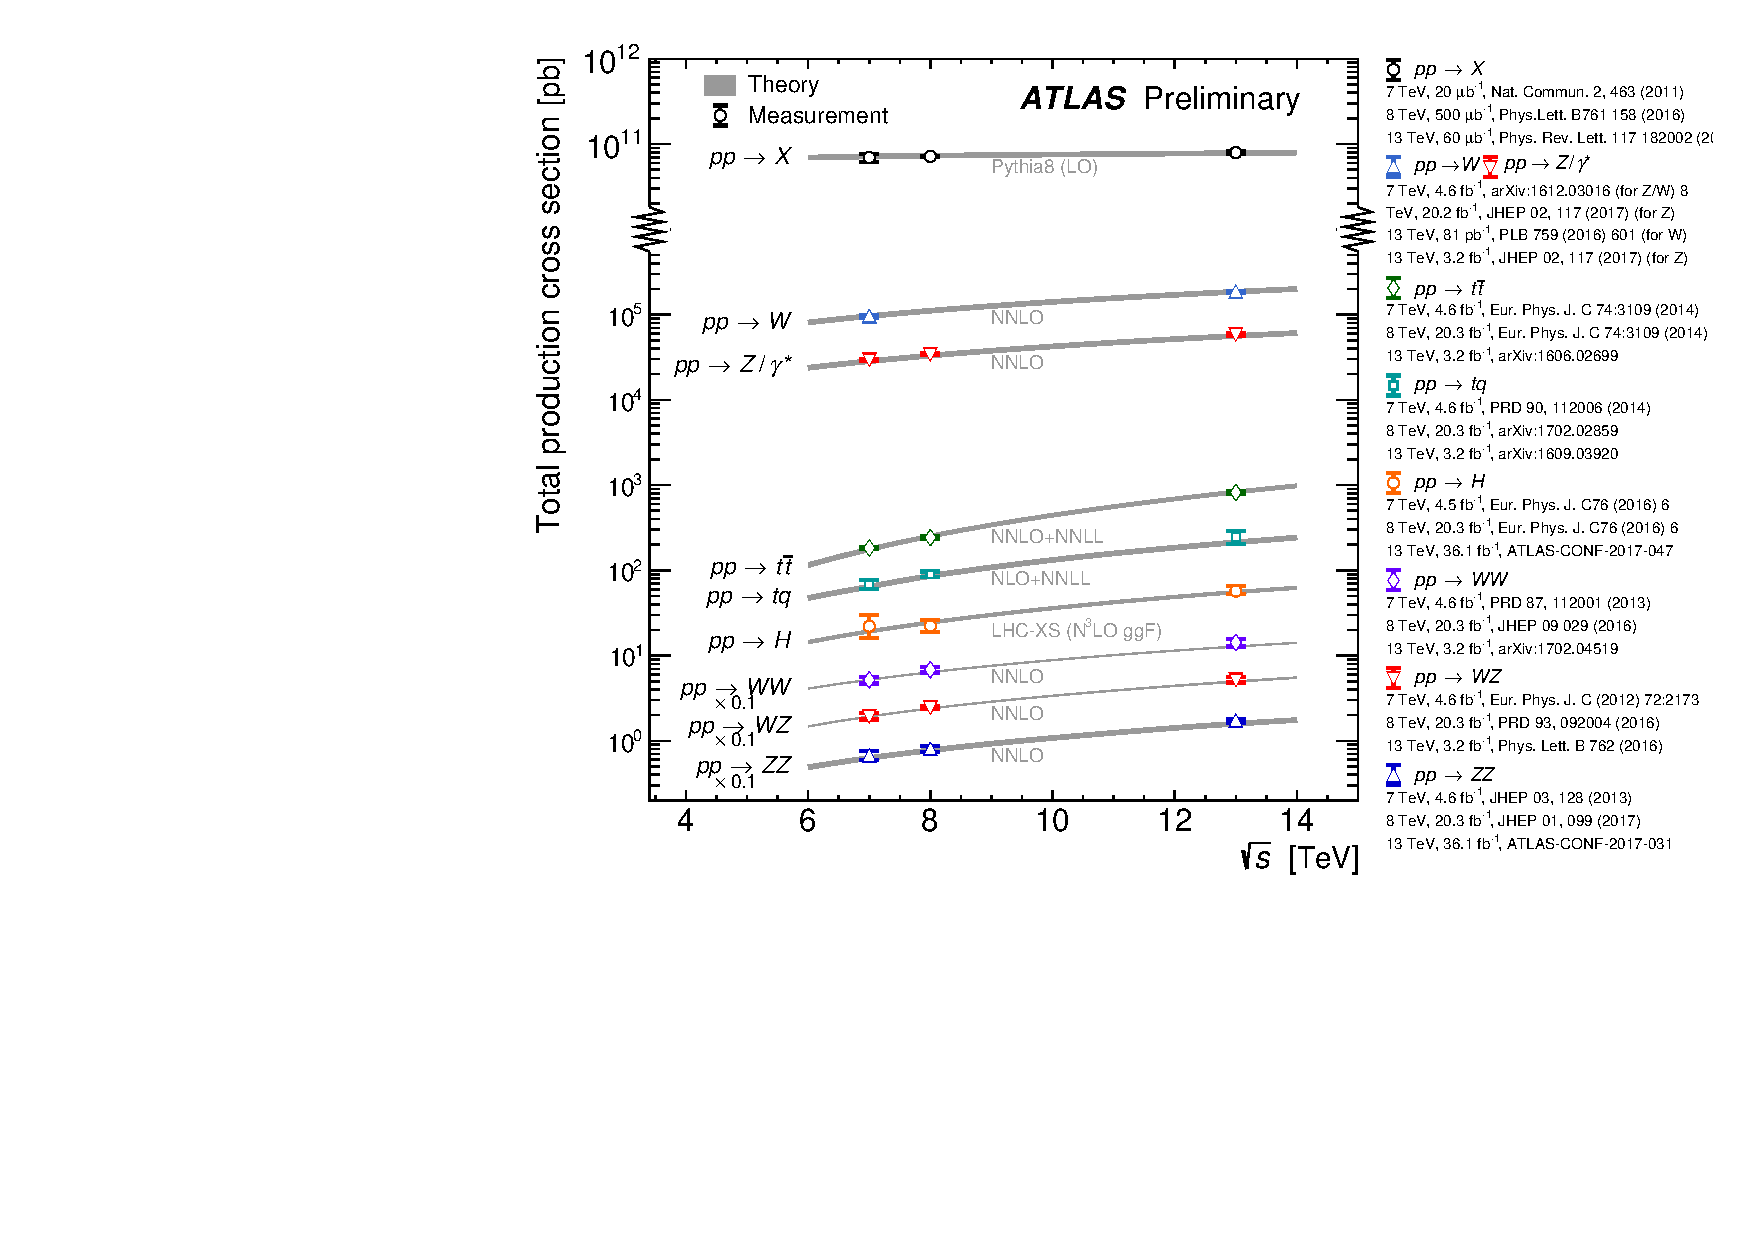
\includegraphics[width=0.7\textwidth]{figures/Theory/ATLAS_n_SMSummary_SqrtS.pdf}
  \caption{Total production cross-section presented by ATLAS as a function of centre-of-mass energy $\sqrt{s}$ from 7 to 13 TeV for some selected processes,
	   the diboson measurements are scaled by a factor 0.1 to allow a presentation without overlaps.}
  \label{fig:diboson_xs1}
\end{figure}

%% ======================================= Vector boson scattering ===================
\textbf{Vector boson scattering}

The $SU(2)_{L} \times U(1)_{Y}$ structure in SM predicts self-interactions between electroweak gauge bosons.
Those self-couplings can involve either three or four gauge bosons at a single vertex, known as triple gauge coupling (\textit{TGC}) and
quartic gauge couplings (\textit{QGC}), repectively.
Vector boson scattering or fusion (\textit{VBS} or \textit{VBF}) is carried out 
by four electroweak vector bosons, namely $Z$, $W^{\pm}$ and photon $(\gamma)$ as the Feynman diagrams shown in figure~\ref{fig:vbs_fd1}. 
And the vertexes include either those self-interactions
or the interactions with Higgs boson described in figure~\ref{fig:vbs_fd2}.
\begin{figure}[!htb]
  \centering
  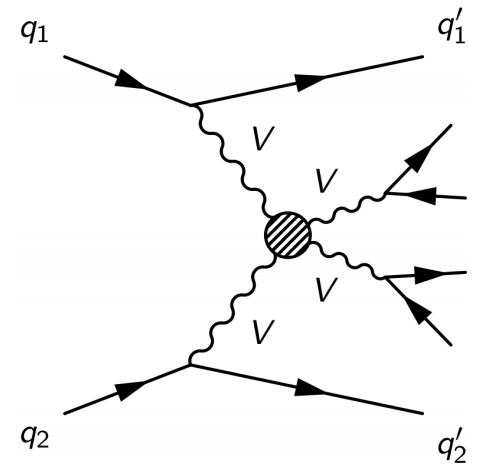
\includegraphics[width=0.4\textwidth]{figures/Theory/VBS.png} 
  \caption{Feynman disgrams of vector boson scattering.}
  \label{fig:vbs_fd1}
\end{figure}
\begin{figure}[!htb]
  \centering
  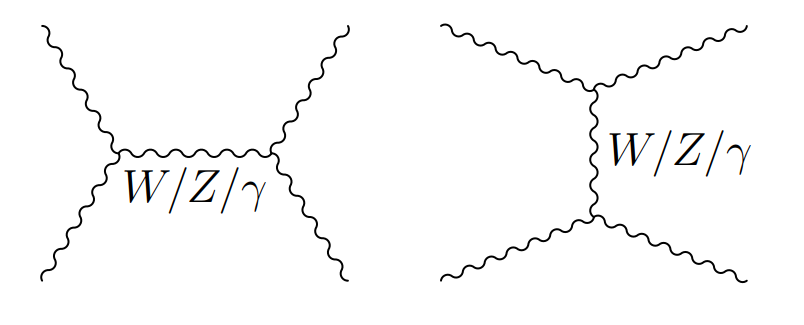
\includegraphics[width=0.6\textwidth]{figures/Theory/vbs_tgc.png} \\
  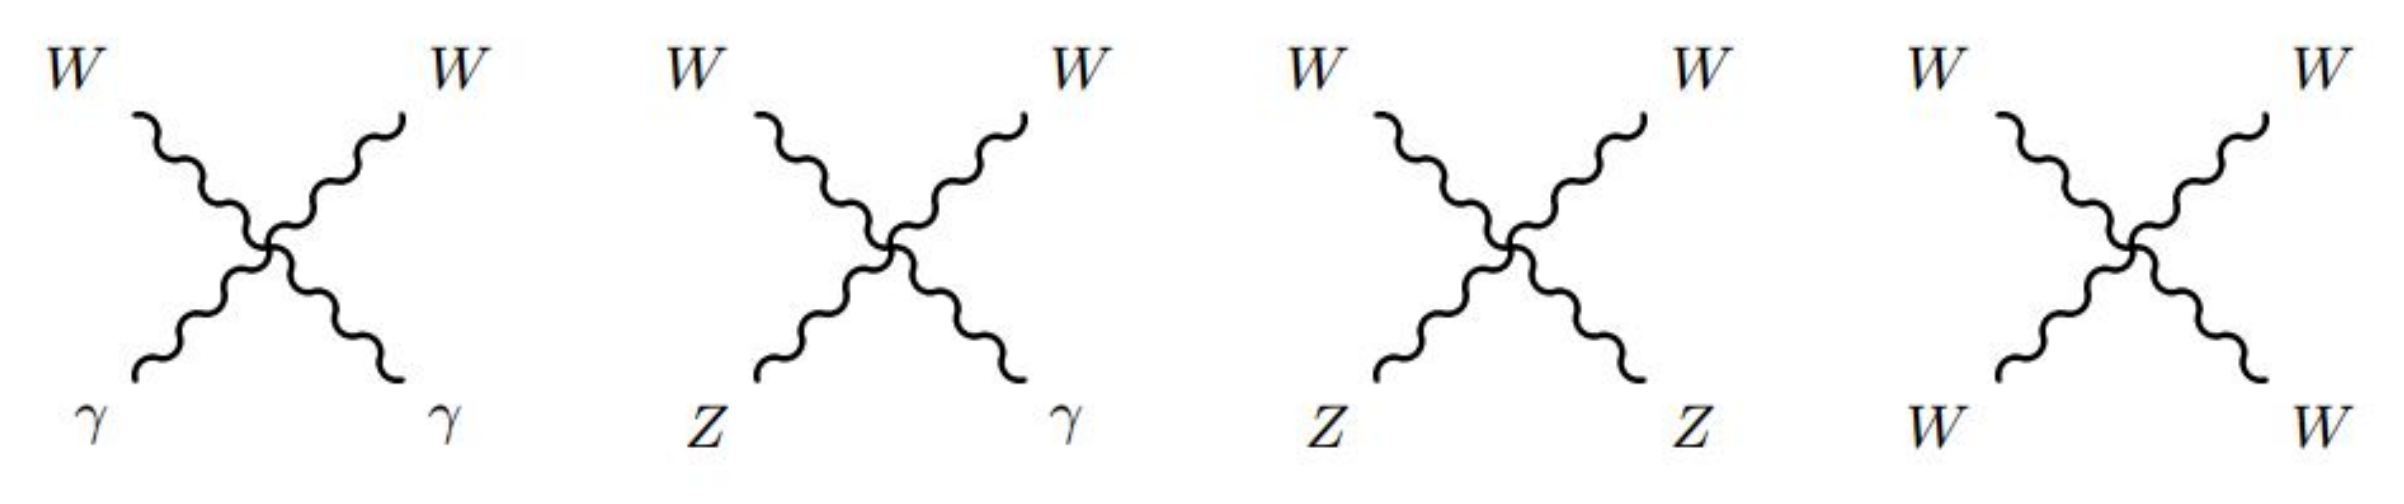
\includegraphics[width=1.0\textwidth]{figures/Theory/vbs_qgc.png} \\
  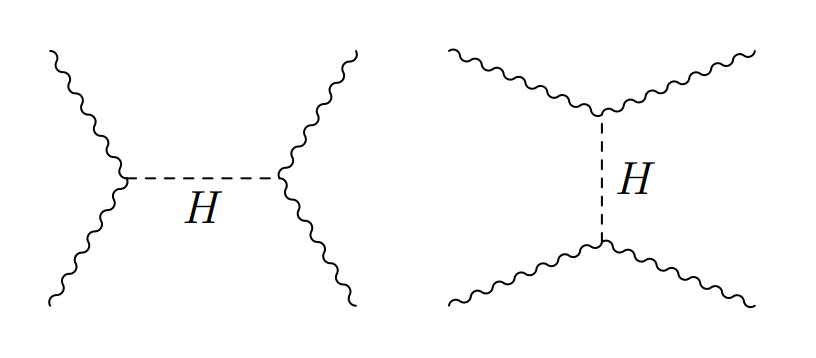
\includegraphics[width=0.6\textwidth]{figures/Theory/vbs_higgs.png} 
  %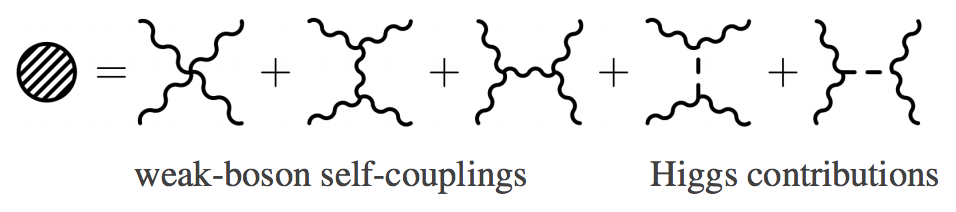
\includegraphics[width=1.0\textwidth]{figures/Theory/VBS_vertex.png}
  \caption{Feynman disgrams of vertexes involving QGC, TGC and Higgs.}
  \label{fig:vbs_fd2}
\end{figure}

The amplitudes of leading-order (LO) VBS can be expressed as:
\begin{equation} \label{eq:amp_tgc}
\begin{split}
	& {iM}_{TGC}^{s-channel} = -i\frac{g_{1}^{2}}{4m_{W}^{4}}[s(t-u)-3m_{W}^{2}(t-u)] \\
	& {iM}_{TGC}^{t-channel} = -i\frac{g_{1}^{2}}{4m_{W}^{4}}\left[t(s-u)-3m_{W}^{2}(s-u)+\frac{8m_{W}^{2}}{s}u^{2}\right]
\end{split}
\end{equation}
\begin{equation}
	{iM}_{QGC} = i\frac{g_{1}^{2}}{4m_{W}^{4}}\left[s^{2}+4st+t^{2}-4m_{W}^{2}(s+t)-\frac{8m_{W}^{2}}{s}ut\right]
\end{equation}
\begin{equation} \label{eq:amp_higgs}
\begin{split}
	{iM}_{Higgs} & = -i\frac{C_{\nu}^{2}g_{1}^{2}}{4m_{W}^{2}}\left[\frac{(s-2m_{W}^{2})^{2}}{s-m_{H}^{2}} + \frac{(t-2m_{W}^{2})^{2}}{t-m_{H}^{2}}\right] \\
                     & \simeq -i\frac{C_{\nu}^{2}g_{1}^{2}}{4m_{W}^{2}}(s+t)
\end{split}
\end{equation}
Combined s- and t-channel of TGC in Eq.~\ref{eq:amp_tgc}:
\begin{equation}
	{iM}_{TGC} = -i\frac{g_{1}^{2}}{4m_{W}^{4}}\left[s^{2}+4st+t^{2}+3m_{W}^{2}t-5m_{W}^{2}s+8m_{W}^{2}\frac{t^{2}}{s}\right]
\end{equation}
Then by combining the QGC term, the amplitude of self-couplings can be written as:
\begin{equation} \label{eq:self_coup}
	{iM}_{TGC} + {iM}_{QGC}= i\frac{g_{1}^{2}}{4m_{W}^{2}}(s+t) + {O}((s/m_{W}^{2})^{0})
\end{equation}
In Eq.~\ref{eq:self_coup}, the amplitude grows as a function of center-of-mass energy ($\sqrt{s}$),
which violates the unitarity in the TeV region.
Considering the Higgs term in Eq.~\ref{eq:amp_higgs} perfectly cancels out this growing,
and the remaining term ${O}((s/m_{W}^{2})^{0})$ depends on the total amplitude in SM.

In conclusion, Higgs boson acts as “moderator” to unitarize high-energy longitudinal vector boson scattering
by restoring unitarity of total amplitude in high energy region.

%\subsection{Diboson physics}

\chapter{The Large Hadron Collider and the ATLAS Detector}

\section{The Large Hadron Collider}
Located near the French-Swiss border at the European Organization for Nuclear Research (CERN),
the Large Hadron Collider (LHC) is the world’s largest and most powerful particle collider.
It's the proton-proton collider with center-of-mass energy up to 14 TeV.
The beams inside the LHC are made to collide at four locations around its 27-kilometer accelerator ring, 
corresponding to the positions of four particle detectors – ATLAS, CMS, ALICE and LHCb.
With its unprecedented energy, the LHC is designed to observe physics that involve highly massive particles
which have never been observable in earlier lower energy accelerators.

\subsection{Operation history and machine layout}

%% ================================= history ==============================
\textbf{Operation history}

The LHC \cite{Bruning:2004ej, Buning:2004wk, Benedikt:2004wm, Evans_2008} 
is a two-ring-superconducting-hadron accelerator and collider lies in a tunnel 27 kilometres in circumference and as deep as 175 metres underground.
It's designed to provide proton-proton (pp) collisions at the centre-of-mass energy ($\sqrt{s}$) up to 14~\tev
with a unprecedented luminosity of $10^{34} cm^{-2} s^{-1}$.
In the meantime, it can also collide heavy (Pb) ions with an energy of 2.8~\tev~ per nucleon and a peak luminosity of $10^{27} cm^{-2} s^{-1}$.
Table~\ref{tab:LHC_parameters} shows the main design parameters of the LHC for proton-proton collisions.
\begin{table}[htbp]
  \centering
  \caption{Summary of design parameters of the LHC for pp collisions.}
  \label{tab:LHC_parameters}
  \begin{tabular}{cc}
    \hline
    Circumference	& 26.7 km\\
    Beam energy at collision	& 7 ~\tev\\
    Beam energy at injection	& 0.45~\tev \\
    Dipole field at 7~\tev	& 8.33 T \\
    Luminosity		& $10^{34} cm^{-2} s^{-1}$ \\
    Beam current	& 0.56 A \\
    Protons per bunch	& $1.1 \times 10^{11}$ \\
    Number of bunches	& 2808 \\
    Nominal bunch spacing	& 24.95 ns \\
    Normalized emittance	& 3.75 $\mu$m \\
    Total crossing angle	& 300 $\mu$rad \\
    Energy loss per turn	& 6.7 keV \\
    Critical synchrotron energy	& 44.1 eV \\
    Radiated power per beam	& 3.8 kW \\
    Stored energy per beam	& 350 MJ \\
    Stored energy in magnets	& 11 GJ \\
    Operating temperature	& 1.9 K \\
    \hline
  \end{tabular}
\end{table}

The LHC was built from 1998 to 2008. 
It started its first beam in September 2008, but then was interrupted by a quench incident only after a few days running.
Then it resumed the operation in November 2009 with a low energy beams.
From March 2010, physics runs took place at the centre-of-mass energy of 7~\tev.
Later on, this energy was increased in 2012 to $\sqrt{s} = 8~\tev$, with an integrated luminosity of 20.3~\ifb, and this period is called "run-1".
After run-1, the LHC was shut down for two years for hardware maintenance and upgrade, starting from February 2013.

The second operation period with higher centre-of-mass energy at 13~\tev~ started from 2015 called "run-2".
And it continued to the end of 2018 with total integrated luminosity reaching about 147 $fb^{-1}$ for ATLAS.
Figure~\ref{fig:lumi_vs_month} shows the cumulative luminosity as a function of time in month delivered to ATLAS experiment during stable beams 
in years from 2011 to 2018.
\begin{figure}[!htb]
  \centering
  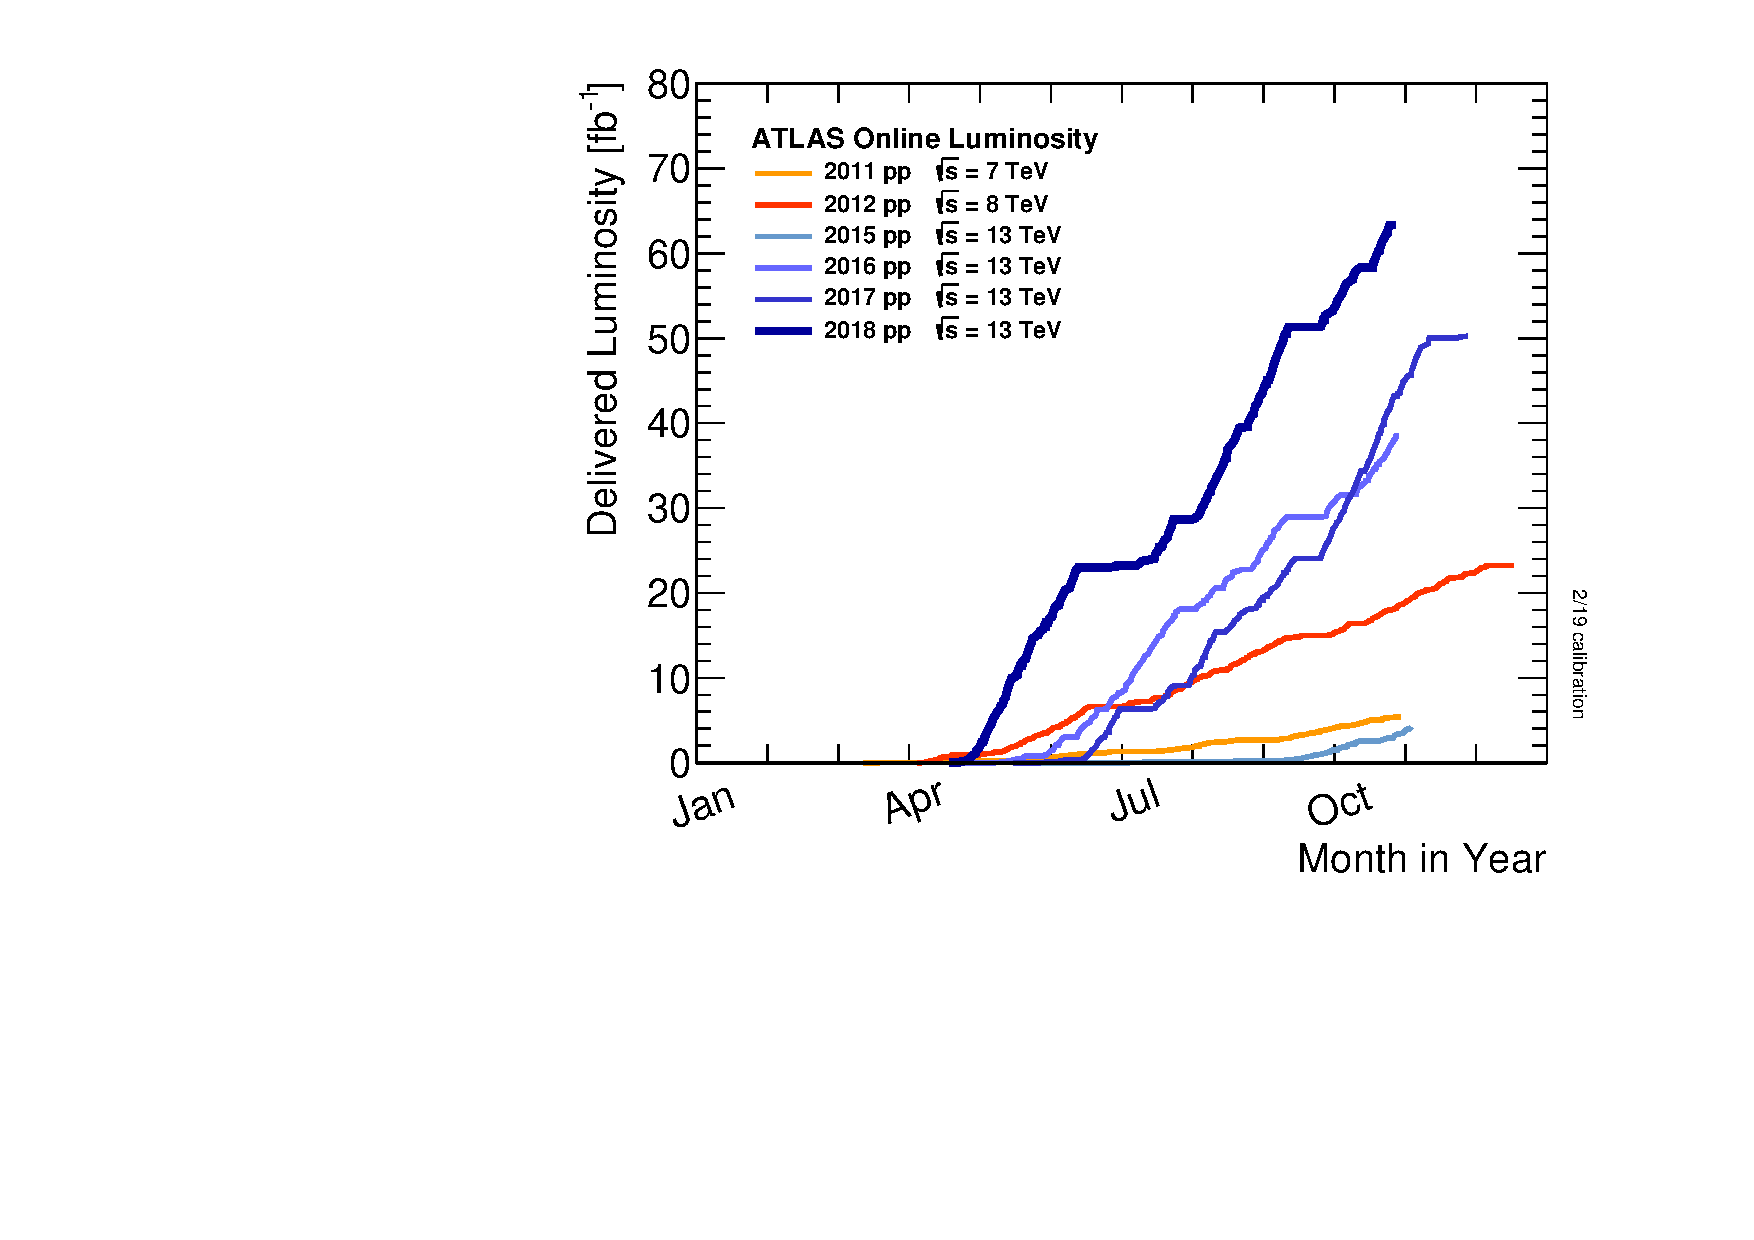
\includegraphics[width=0.6\textwidth]{figures/Detector/intlumivsyear.pdf}
  \caption{Cumulative luminosity as a function of time in years from 2011 to 2018 for ATLAS detector.}
  \label{fig:lumi_vs_month}
\end{figure}

%% ======================================= layout ==============================
\textbf{Machine layout}

The layout of CERN accelerator complex is shown in figure~\ref{cern_layout}.
The protons are accelerated by a series of machines before being injected into the main cavity.
At beginning, the 50~\mev~ protons are produced in the linear particle accelerator LINAC2, 
and then further accelerated to 1.4~\gev~ in Proton Synchrotron Booster (PSB).
The protons are then injected into the Proton Synchrotron (PS) to gain the energy of 26~\gev~ and further accelerated to 450~\gev~ in Super Proton Synchrotron (SPS).
At the end, they are injected into the main ring, and can reach a maximum energy of 7~\tev.

\begin{figure}[!htb]
  \centering
  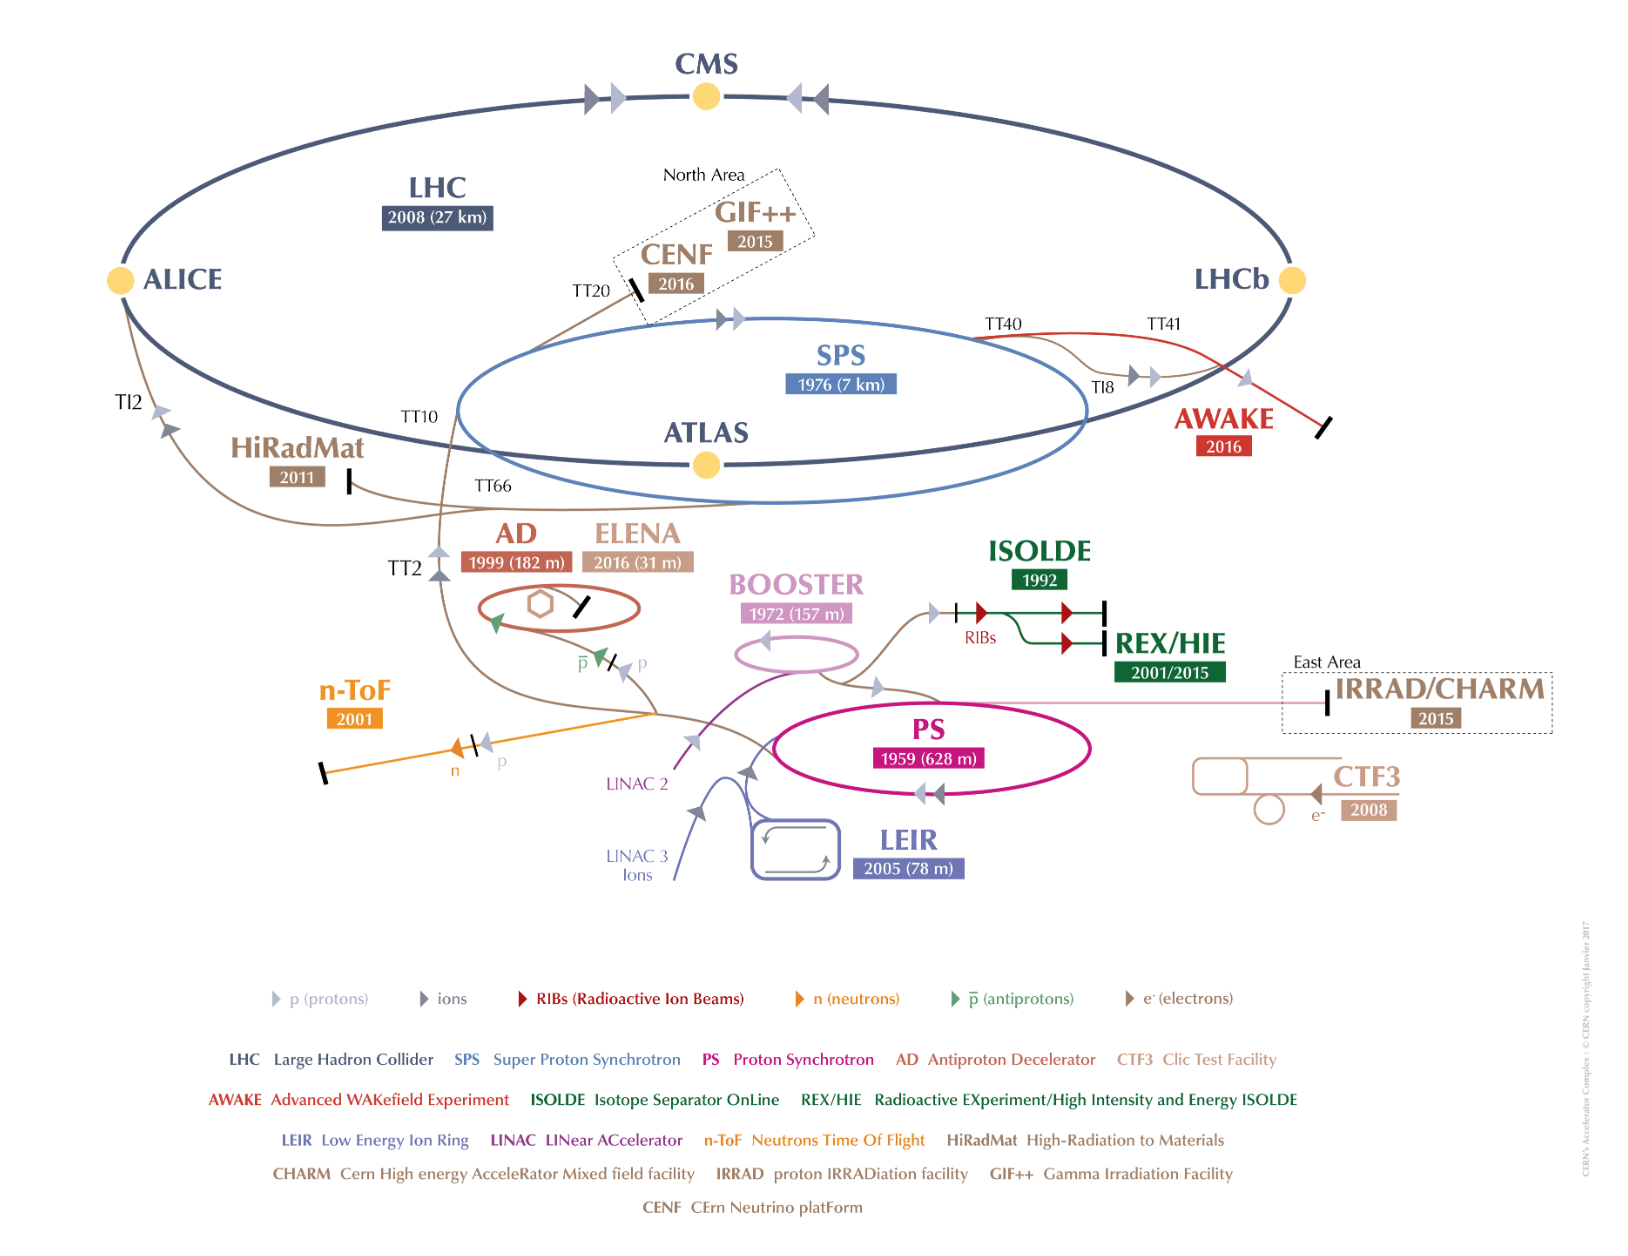
\includegraphics[width=1.0\textwidth]{figures/Detector/LHC_v2017.png}
  \caption{CERN accelerator complex \cite{Mobs:2197559}.}
  \label{cern_layout}
\end{figure}

The collisions can occur in 4 points, with corresponding 4 major detector experiments that are briefly described as follows:
\begin{itemize}
	\item \textbf{ATLAS}: A Toroidal LHC ApparatuS, one of the two general-purpose particle detector experiments and detector with largest volume at the LHC. It is designed to search for the Higgs boson, test the stardand model of particle physics and search for possible beyond SM physics.
	\item \textbf{CMS}: Compact Muon Solenoid, another large general-purpose particle physics detector, with the same physics goal (also cross check) as ATLAS.
	\item \textbf{ALICE}: A Large Ion Collider Experiment, it is optimized to study heavy-ion (Pb-Pb nuclei) collisions at a centre-of-mass energy of 2.76~\tev~ per nucleon pair.
	\item \textbf{LHCb}: Large Hadron Collider beauty, it is a specialized b-physics experiment, designed primarily to measure the parameters of CP violation in the interactions of b-hadrons.
\end{itemize}



%\subsection{Operation history and machine layout}
\subsection{Luminosity and pile-up}

\textbf{Luminosity}

In beam–beam collisions, the event rate for a process is written as~\cite{Evans_2008}:
\begin{equation}
	N = \mathcal{L} \sigma
\end{equation}
where $\sigma$ is the cross section of the process, and $\mathcal{L}$ is the luminosity.
To study rare events, $\mathcal{L}$ must be as high as possible.
The luminosity only depends on the beam parameters as:
\begin{equation} \label{eq:lumi}
	\mathcal{L} = \frac{ N_{b}^{2} n f_{r} \gamma}{4\pi \epsilon_{n} \beta^{*}}
\end{equation}
in which $N_{b}$ represents the number of particles per bunch, $n$ denotes the number of bunches per beam,
$f_{r}$ is the revolution frequency, and $\gamma$ is relativistic $\gamma$ factor, 
$\epsilon_{n}$ is the normalized transverse emittance and $\beta^{*}$ denotes the $\beta$ function at the collision point.
To reduce the beam-beam interaction effects, the bunches must have a crossing angle,
which produces a geometrical luminosity reduction factor $F$:
\begin{equation}
	F = 1 / \sqrt{1 + \left( \frac{\theta_{c}\sigma_{Z}}{2\sigma^{*}} \right) }
\end{equation}
where $\theta_{c}$ denotes the crossing angle at the interaction point, $\sigma_{Z}$ is the root mean square (RMS) bunch length
and $\sigma^{*}$ is the transverse RMS beam size at crossing point.

The luminosity expressed in Eq.~\ref{eq:lumi} is normally the instantaneous luminosity.
In fact the running conditions usually vary with time, so the luminosity can change as well.
To take into account the time dependence, integrated luminosity is invited, by integraling the instantaneous luminosity over time:
\begin{equation}
	L = \int \mathcal{L}(t) dt
\end{equation}
The unit of integrated luminosity we commonly use is $b^{-1}$ that satisfying $1 b^{-1} = 10^{24} cm^{-2}$.
Figure~\ref{fig:lumi_vs_time} shows integrated luminosity as a function of time delivered to ATLAS (green), 
recorded by ATLAS (yellow), and certified to be good quality data (blue) during run-2 pp collisions.
For most physics analysis, the data with good quality (require to satisfy \textit{Good Run List}) is used.
\begin{figure}[!htb]
  \centering
  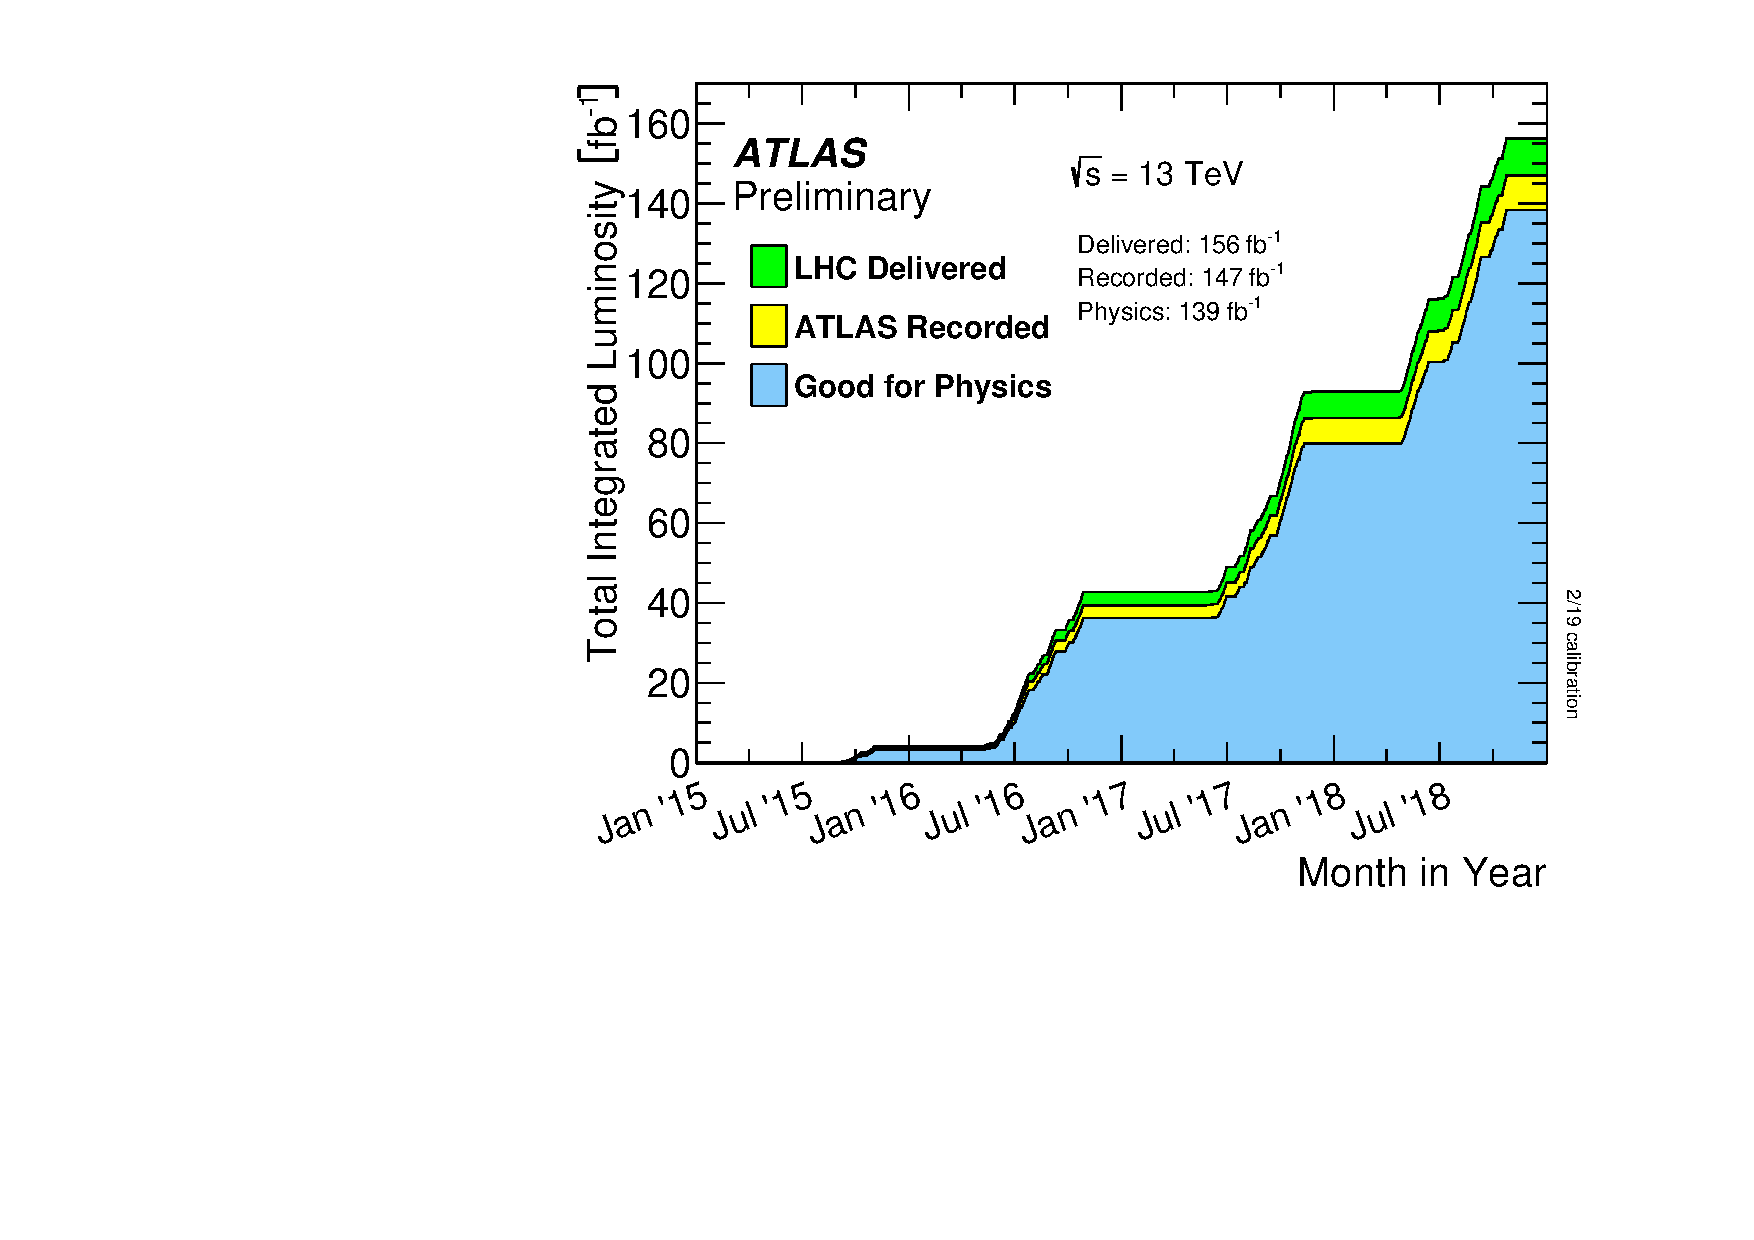
\includegraphics[width=0.6\textwidth]{figures/Detector/intlumivstimeRun2DQall.pdf}
  \caption{Integrated luminosity vs delivered month from 2015 to 2018 in ATLAS experiment.}
  \label{fig:lumi_vs_time}
\end{figure}

\textbf{Pile-up}

In collisions, multiple interactions can happen in one single bunch crossing, which is called ``\textit{pile-up}".
The variable $\left< \mu \right>$, representing the average number of interactions per bunch crossing that used to describe pile-up effect, is defined as:
\begin{equation}
    \left< \mu \right> = \frac{\mathcal{L}_{tot}\sigma}{f_{r}n_{bunch}}
\end{equation}
where $\mathcal{L}_{tot}$ is the instantaneous luminosity, $\sigma$ denotes the inelastic cross section,
$f_{r}$ represents the LHC revolution frequency and $n_{bunch}$ is the number of colliding bunches.
Usually, with increasing luminosity, the pile-up becomes more significant.
Figure~\ref{fig:run2_mu} shows the luminosity-weighted distribution of the mean number of interactions per crossing
for pp collision data from 2015 to 2018 (full run-2), the challenge of pile-up increased in each year.
\begin{figure}[!htb]
  \centering
  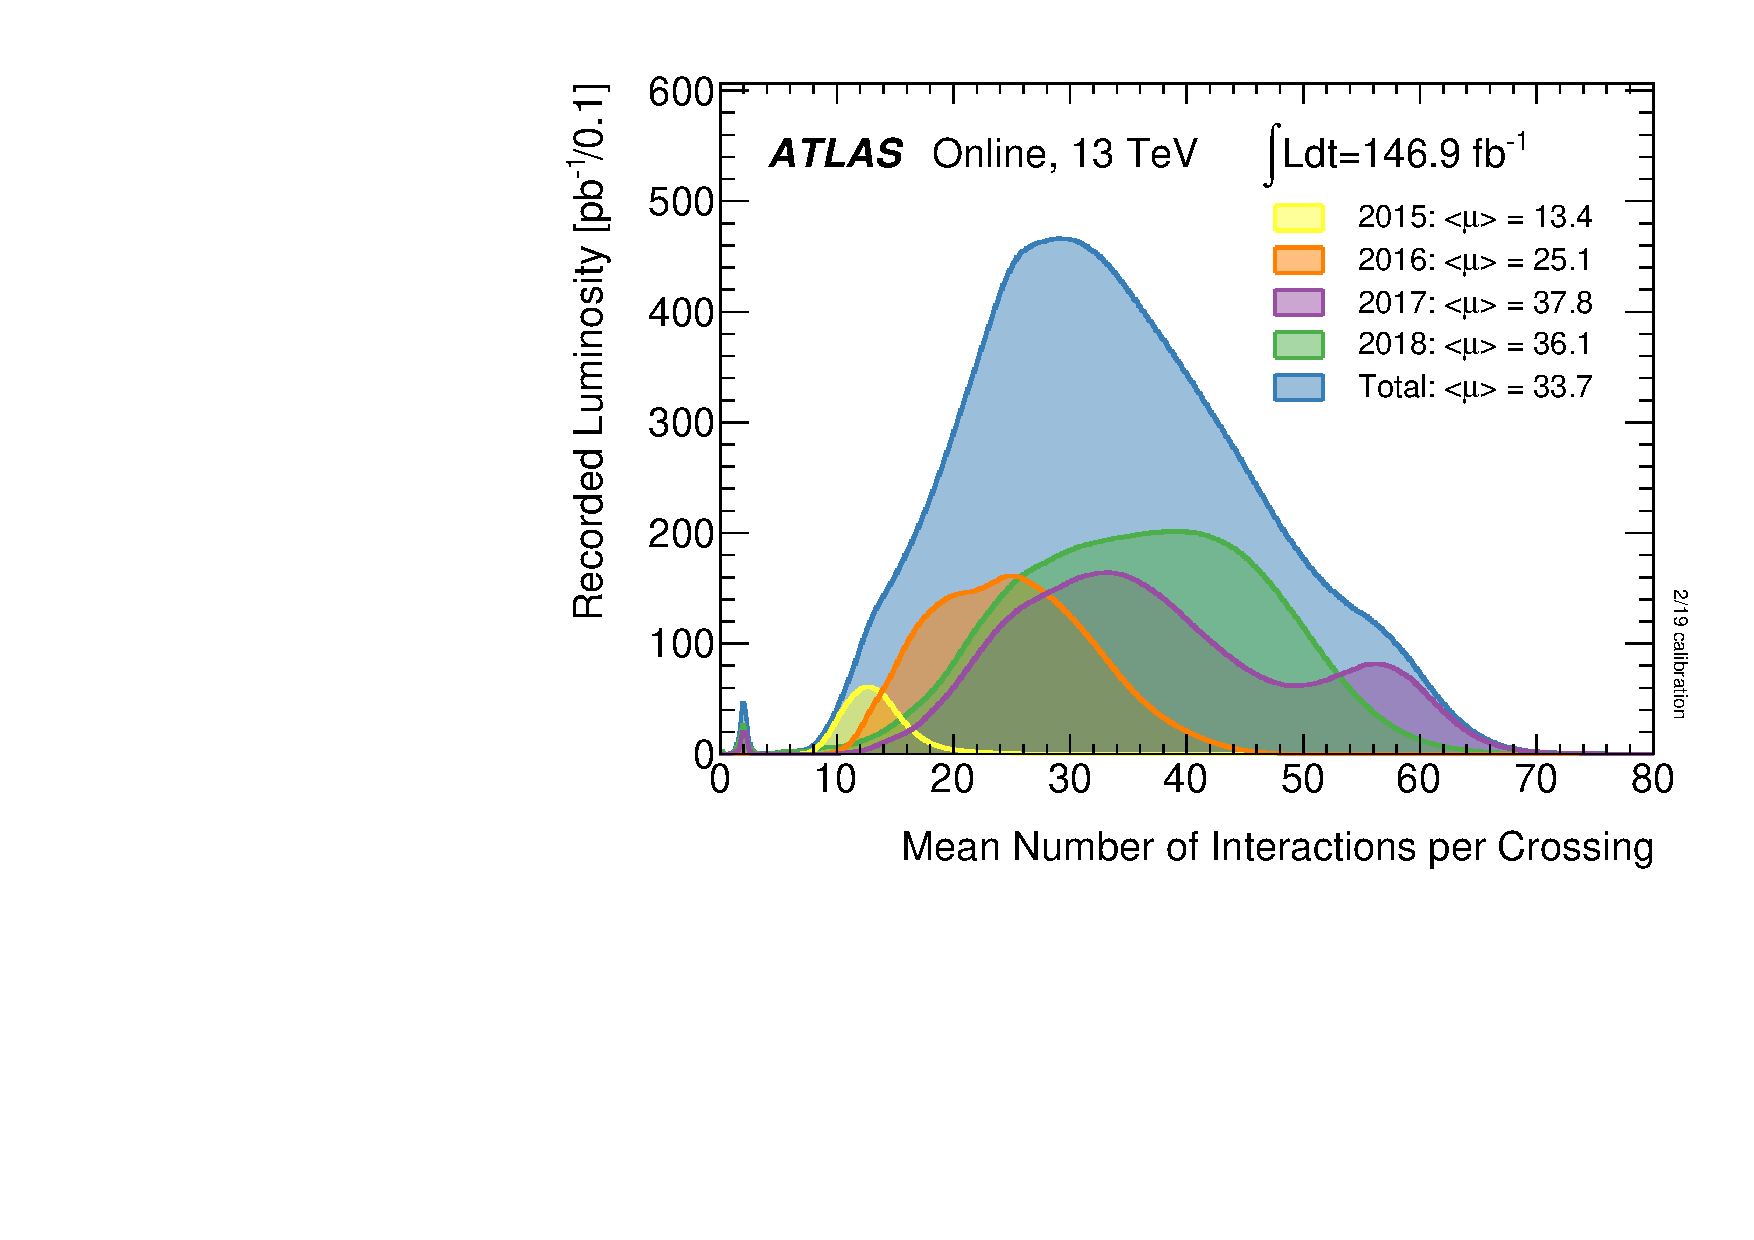
\includegraphics[width=0.6\textwidth]{figures/Detector/mu_2015_2018.pdf}
  \caption{Number of interactions per crossing weighted bt luminosity from 2015 to 2018 in ATLAS experiment.}
  \label{fig:run2_mu}
\end{figure}

%\subsection{Luminosity and pile-up}

\section{ATLAS detector}
\subsection{Detector overview}

ATLAS is the world's largest volume particle detector.
It is a cylinder with 46 meters long, 25 meters in diameter, and sits in a cavern 100 meters below ground.
The detector contains about 3000 km of cables and it weights 7000 tonnes.

The coordinate system and nomenclature used to describe the ATLAS detector \cite{Collaboration_2008} is depicted in figure~\ref{fig:coordinate}. We define the nominal interaction point as the origin of the coordinate system, the beam direction as the \textit{z}-axis and the \textit{x-y} plane is transverse to the beam direction.
The positive \textit{x}-axis is given as the direction from interaction point to the centre of the LHC ring, 
while the positive \textit{y}-axis points upward.
\begin{figure}[!htb]
  \centering
  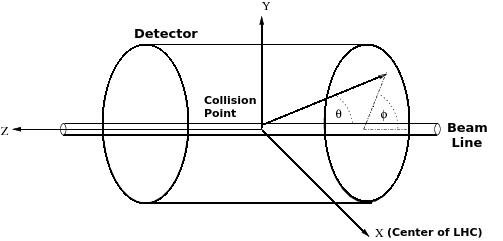
\includegraphics[width=0.9\textwidth]{figures/Detector/Coordinate_system_atlas.png}
  \caption{Coordinate system used by the ATLAS experiment at the LHC \cite{Perez:phdthesis}.}
  \label{fig:coordinate}
\end{figure}
There are two sides of detector A and C, in which A (C) -side is in the positive (negative) \textit{z} direction.
The polar angle $\theta$ is measured from the beam axis, while the azimuthal angle $\phi$ is obtained around the beam axis.
In physics analysis, we usually use the pseudorapidity $\eta$ designed as:
\begin{equation}
    \eta = - ln \left[ tan\left( \frac{\theta}{2}\right) \right]
\end{equation}
instead of $\theta$ angle. 
And for massive objects (eg. jets), the rapidity is used:
\begin{equation}
    y = \frac{1}{2} ln \left[ \frac{E+p_{z}}{E-p_{z}} \right]
\end{equation}

In addition, the transverse momentum $p_{T}$, transverse energy $E_{T}$ and the missing transverse energy $E_{T}^{miss}$ are defined in \textit{x-y} plane.
The $\Delta R$, a commonly used distance measurement, is defined in the pseudorapidity-azimuthal angle space as:
\begin{equation}
    \Delta R = \sqrt{ \Delta\eta^{2} + \Delta\phi^{2}}.
\end{equation}

The overall ATLAS layout is shown in figure~\ref{fig:atlas_layout}, which is forward-backward symmetric with respect to the interaction point.
\begin{figure}[!htb]
  \centering
  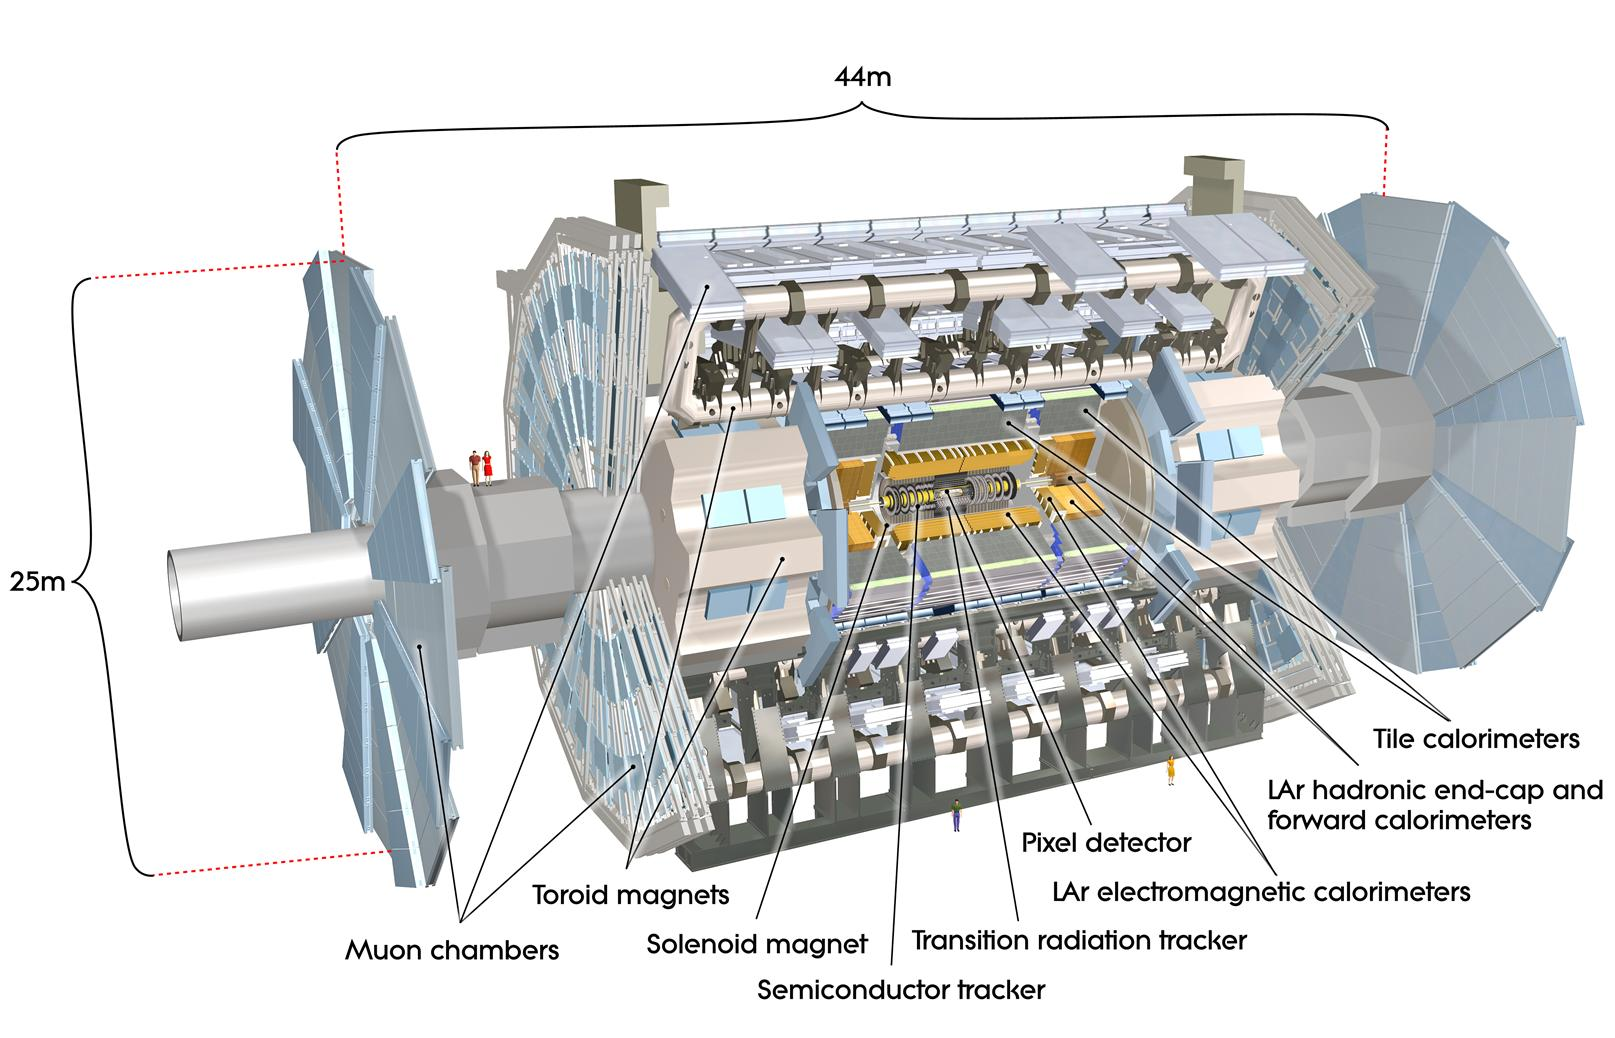
\includegraphics[width=1.0\textwidth]{figures/Detector/atlas_layout.jpg}
  \caption{Layout view of the ATLAS detector \cite{Pequenao:1095924}.}
  \label{fig:atlas_layout}
\end{figure}
The magnet configuration has a thin superconducting-solenoid surrounding the inner-detector, 
and three large superconducting-toroids (one barrel and two end-caps) around the calorimeters.

\textbf{The inner detector}, which is the innermost part of ATLAS, is surrounded by a 2 T solenoidal magnetic field.
It's used for pattern recognition, momentum and vertex measurements and electron identification, with the combination of tracking system in the region of $\eta$ up to 2.5.

\textbf{The calorimeter} is outside the solenoid, for electromagnetic and hadronic energy measurements.
The high granularity liquid-argon (LAr) electromagnetic sampling calorimeters is used to measure energy and position with range up to $|\eta| < 3.2$ for electrons and photons.
For hadron, a scintillator-tile calorimeter is used in the range of $|\eta| < 1.7$, and the liquid-argon hadronic endcap calorimeters (HEC) is used in end-cap region.
And then the LAr forward calorimeters provide both electromagnetic and hadronic energy measurements with the coverage in forward region up to $|\eta| = 4.9$.

\textbf{The muon spectrometer} is the outermost layer.
It's a air-core toroid system, with a long barrel and two inserted end-cap magnets that provides strong bending power in a large volume within a light and open structure.
A set of chambers measuring the tracks of muons with high spatial precision and accurate time-resolution are used.
Multiple-scattering effects are minor, and excellent muon momentum resolution can be achieved.

%\subsection{Dector overview}

%% !TeX root = ../main.tex

\chapter{引用文献的标注}

模板使用 \pkg{natbib} 宏包来设置参考文献引用的格式,
更多引用方法可以参考该宏包的使用说明。



\section{顺序编码制}

\subsection{角标数字标注法}

\citestyle{super}
\noindent
\begin{tabular}{l@{\quad$\Rightarrow$\quad}l}
  \verb|\cite{knuth86a}|         & \cite{knuth86a}         \\
  \verb|\citet{knuth86a}|        & \citet{knuth86a}        \\
  \verb|\cite[42]{knuth86a}|     & \cite[42]{knuth86a}     \\
  \verb|\cite{knuth86a,tlc2}|    & \cite{knuth86a,tlc2}    \\
  \verb|\cite{knuth86a,knuth84}| & \cite{knuth86a,knuth84} \\
\end{tabular}


\subsection{数字标注法}

\citestyle{numbers}
\noindent
\begin{tabular}{l@{\quad$\Rightarrow$\quad}l}
  \verb|\cite{knuth86a}|         & \cite{knuth86a}         \\
  \verb|\citet{knuth86a}|        & \citet{knuth86a}        \\
  \verb|\cite[42]{knuth86a}|     & \cite[42]{knuth86a}     \\
  \verb|\cite{knuth86a,tlc2}|    & \cite{knuth86a,tlc2}    \\
  \verb|\cite{knuth86a,knuth84}| & \cite{knuth86a,knuth84} \\
\end{tabular}



\section{著者-出版年制标注法}

\citestyle{authoryear}
\noindent
\begin{tabular}{l@{\quad$\Rightarrow$\quad}l}
  \verb|\cite{knuth86a}|         & \cite{knuth86a}         \\
  \verb|\citep{knuth86a}|        & \citep{knuth86a}        \\
  \verb|\cite[42]{knuth86a}|     & \cite[42]{knuth86a}     \\
  \verb|\cite{knuth86a,tlc2}|    & \cite{knuth86a,tlc2}    \\
  \verb|\cite{knuth86a,knuth84}| & \cite{knuth86a,knuth84} \\
\end{tabular}

\vskip 2ex \citestyle{super}
注意,参考文献列表中的每条文献在正文中都要被引用
\cite{slg,lyc,ljs,cgw,cjb,kqy,yhs,yx,dwx,jxz,wjk,syw,wf,xd,twh,huston}。

\bibliography{bib/reference}

\appendix
%% !TeX root = ../main.tex

\chapter{补充材料}


补充内容。


\backmatter
%% !TeX root = ../main.tex

\begin{publications}

\section*{已发表论文}

\begin{enumerate}
    \item ATLAS Collaboration. Search for electroweak diboson production in association with a high-mass dijet system in semileptonic final states in pp collisions at 13TeV with the ATLAS detector[J]. \textbf{Phys. Rev. D 100, 032007}.
    \item ATLAS Collaboration. Constraints on off-shell Higgs boson production and the Higgs boson total width in $ZZ \rightarrow \llll$ and $ZZ \rightarrow \llvv$ final states with the ATLAS detector[J]. \textbf{Physics Letters B, 2018, 786}.
    \item ATLAS Collaboration. Measurement of the four-lepton invariant mass spectrum in 13~\tev~ proton-proton collisions with the ATLAS detector[J]. \textbf{Journal of High Energy Physics, 2019, 2019(4): 48}.
    \item Chen K, et al. Design and Evaluation of the LAr Trigger Digitizer Board in the ATLAS Phase-I Upgrade[J]. \textbf{IEEE Transactions on Nuclear Science, 2019, 66(8): 2011-2016}.
\end{enumerate}

\section*{待发表论文}

\begin{enumerate}
    \item Observation of electroweak production of two jets and a Z-boson pair with the ATLAS detector at the LHC. \textbf{Submitted to Nature Physics, e-print: arXiv:2004.10612}.
    \item Search for heavy resonances decaying into a pair of Z bosons in $ZZ \rightarrow \llll$ and $ZZ \rightarrow \llvv$ final states using 139~\ifb~ of pp collisions at 13~\tev~ with the ATLAS detector. \textbf{Submitted to Eur. Phy. J. C, e-print: arXiv:2009.14791}.
\end{enumerate}

\section*{会议报告}
\begin{enumerate}
    \item Measurement of Inclusive \llll and \llvv + 2-jet Cross Section and Observation of EW Component in 13~\TeV~ Proton-Proton Collisions with the ATLAS detector. \textbf{Workshop on Connecting Insights in Fundamental Physics: Standard Model and Beyond, Corfu, Greece, 2019.9}
    \item Off-shell Higgs signal strength measurement in the high-mass $ZZ \rightarrow \llll$ and $ZZ \rightarrow \llvv$ final states with the ATLAS detector. \textbf{American Physics Society April Meeting, Columbus, USA, 2018.4}
\end{enumerate}

\end{publications}


\end{document}
